\documentclass[conference]{IEEEtran}
\IEEEoverridecommandlockouts
\usepackage[T1]{fontenc}
\usepackage[utf8]{inputenc}
\usepackage{cite}
\usepackage{amsmath,amssymb}
\usepackage{graphicx}
\usepackage{booktabs}
\usepackage{longtable}
\usepackage{array}
\usepackage{xcolor}
\usepackage{url}
\usepackage[hidelinks]{hyperref}
\graphicspath{{figures/}}
% Auto-generated by paper/tools/build_facts.py from the result JSONs. Do not edit by hand.
\newcommand{\fullRows}{46,775,660}
\newcommand{\fullFeat}{39}
\newcommand{\fullBenign}{1,098,126}
\newcommand{\fullAttack}{45,677,534}
\newcommand{\vfRows}{7,845,673}
\newcommand{\vfTrain}{5,962,711}
\newcommand{\vfVal}{313,827}
\newcommand{\vfTest}{1,569,135}
\newcommand{\vfBenign}{184,766}
\newcommand{\vfAttack}{7,660,907}
\newcommand{\vtVal}{2,339,084}
\newcommand{\vtTest}{9,350,212}
\newcommand{\vtTrain}{35,086,364}
\newcommand{\fullBestAccTwo}{0.9937}
\newcommand{\fullBestMfTwo}{0.9339}
\newcommand{\fullBestAccEight}{0.8410}
\newcommand{\fullBestMfEight}{0.7324}
\newcommand{\fullBestAccThirtyFour}{0.7895}
\newcommand{\fullBestMfThirtyFour}{0.6452}
\newcommand{\paperAccTwo}{0.9968}
\newcommand{\paperMfTwo}{0.9653}
\newcommand{\msAccTwo}{0.9938}
\newcommand{\msAccSdTwo}{0.000003}
\newcommand{\msMfTwo}{0.9328}
\newcommand{\msMfSdTwo}{0.000030}
\newcommand{\paperAccEight}{0.9944}
\newcommand{\paperMfEight}{0.7193}
\newcommand{\msAccEight}{0.8408}
\newcommand{\msAccSdEight}{0.000060}
\newcommand{\msMfEight}{0.7317}
\newcommand{\msMfSdEight}{0.000056}
\newcommand{\paperAccThirtyFour}{0.9916}
\newcommand{\paperMfThirtyFour}{0.7140}
\newcommand{\msAccThirtyFour}{0.7945}
\newcommand{\msAccSdThirtyFour}{0.000073}
\newcommand{\msMfThirtyFour}{0.6434}
\newcommand{\msMfSdThirtyFour}{0.000157}
\newcommand{\vfAAccTwo}{0.9972}
\newcommand{\vfAMfTwo}{0.9696}
\newcommand{\vfBAccTwo}{0.9977}
\newcommand{\vfBMfTwo}{0.9754}
\newcommand{\vfCAccTwo}{0.9947}
\newcommand{\vfCMfTwo}{0.9436}
\newcommand{\vfDAccTwo}{0.9959}
\newcommand{\vfDMfTwo}{0.9562}
\newcommand{\vfAAccEight}{0.9961}
\newcommand{\vfAMfEight}{0.8799}
\newcommand{\vfBAccEight}{0.9967}
\newcommand{\vfBMfEight}{0.8925}
\newcommand{\vfCAccEight}{0.9076}
\newcommand{\vfCMfEight}{0.7346}
\newcommand{\vfDAccEight}{0.9154}
\newcommand{\vfDMfEight}{0.7547}
\newcommand{\vfAAccThirtyFour}{0.9951}
\newcommand{\vfAMfThirtyFour}{0.8361}
\newcommand{\vfBAccThirtyFour}{0.9957}
\newcommand{\vfBMfThirtyFour}{0.8484}
\newcommand{\vfCAccThirtyFour}{0.8900}
\newcommand{\vfCMfThirtyFour}{0.6979}
\newcommand{\vfDAccThirtyFour}{0.8976}
\newcommand{\vfDMfThirtyFour}{0.7143}
\newcommand{\nOneTwin}{59.05\%}
\newcommand{\nOneDDoS}{67.61\%}
\newcommand{\nOneBenign}{0.54\%}
\newcommand{\nOneInfl}{-0.0176}
\newcommand{\nOneTwinMf}{0.6130}
\newcommand{\nOneNonTwinMf}{0.7292}
\newcommand{\vfTwin}{5.61\%}
\newcommand{\vfDup}{3.51\%}
\newcommand{\nTwoAMf}{0.7308}
\newcommand{\nTwoAAcc}{0.8415}
\newcommand{\nTwoBMf}{0.7297}
\newcommand{\nTwoBAcc}{0.8572}
\newcommand{\nTwoCMf}{0.4454}
\newcommand{\nTwoCAcc}{0.7455}
\newcommand{\nTwoDMf}{0.4557}
\newcommand{\nTwoDAcc}{0.7217}
\newcommand{\nTwoDrop}{0.2751}
\newcommand{\nTwoDedupPct}{54.65\%}
\newcommand{\nThreeShare}{95.18\%}
\newcommand{\nThreeFloodAcc}{0.9923}
\newcommand{\nThreeFloodMf}{0.7660}
\newcommand{\nThreeEightAcc}{0.8410}
\newcommand{\nThreeEightMf}{0.7324}
\newcommand{\nThreeBinPaper}{0.8561}
\newcommand{\nThreeBinGroup}{0.8081}
\newcommand{\vfDdWith}{285}
\newcommand{\vfDdWithShare}{5.47\%}
\newcommand{\vfDdNo}{123,149}
\newcommand{\vfDdNoShare}{92.82\%}
\newcommand{\vfDdNoA}{133,657}
\newcommand{\iatAcc}{0.9905}
\newcommand{\iatMf}{0.8194}
\newcommand{\iatMaj}{0.7278}
\newcommand{\iatSecondName}{Min}
\newcommand{\iatSecondAcc}{0.8111}
\newcommand{\iatSecondMf}{0.3892}
\newcommand{\iatImpEight}{39.55\%}
\newcommand{\nFourDrop}{0.000532}
\newcommand{\nFourBase}{0.9934}
\newcommand{\nFiveAcc}{99.9997\%}
\newcommand{\nFiveMfChange}{-0.0184}
\newcommand{\hierMf}{0.6352}
\newcommand{\hierMfSd}{0.000102}
\newcommand{\flatMfThirtyFour}{0.6429}
\newcommand{\cbBestMf}{0.5417}
\newcommand{\cbBestName}{catboost\_c1\_none\_s2}
\newcommand{\focalMf}{0.5152}
\newcommand{\nSixBestP}{0.25}
\newcommand{\nSixBestMf}{0.7285}
\newcommand{\idsRows}{200,000}
\newcommand{\idsActAcc}{0.99448}
\newcommand{\idsEightAcc}{0.91522}
\newcommand{\idsEightMf}{0.7604}
\newcommand{\idsFalseBlock}{2.65\%}
\newcommand{\idsFalseBlockN}{124}
\newcommand{\idsMiss}{0.29\%}
\newcommand{\idsMissN}{567}
\newcommand{\idsErr}{16,956}
\newcommand{\idsAbsorbed}{15,852}
\newcommand{\idsAbsorbedDd}{15,758}
\newcommand{\idsLatSingle}{1.46}
\newcommand{\idsLatSingleP}{4.10}
\newcommand{\idsLatBatch}{0.0363}
\newcommand{\idsLatBatchP}{0.0424}
\newcommand{\nModels}{92}
\newcommand{\nPosthoc}{20}
\newcommand{\nModelsVfour}{30}
\newcommand{\iatMedDoSTCP}{8.295e+07}
\newcommand{\iatMedDDoSICMP}{8.313e+07}
\newcommand{\iatMedBenign}{1.665e+08}
 % every number in the text comes from here (generated from the result JSONs)

\begin{document}

\title{Beating a Benchmark Is Not Detecting Attacks: Leakage, Timestamp Proxies and a Deployable
Intrusion Prevention Layer for CICIoT2023}

\author{\IEEEauthorblockN{Saksham Kala}
\IEEEauthorblockA{Department of Computer Science and Engineering\\
Bennett University, Greater Noida, India\\
B.Tech CSE (2023--2027)}}

\maketitle

\begin{abstract}
CICIoT2023 is a large IoT intrusion detection benchmark on which many studies, including its authors' Random
Forest (RF) baseline, report accuracies around 99\%. We trained \nModels{} models (RF, LightGBM, XGBoost and CatBoost on
GPU, an MLP, focal-loss XGBoost and a hierarchical 8$\rightarrow$34 classifier) plus post-hoc thresholding,
calibration and stacking, with all selection done on a validation split. On the full 39-feature release
(\fullRows{} rows) we beat the published 8-class macro-F1 (\fullBestMfEight{} vs \paperMfEight{}) but not
2-class accuracy (\fullBestAccTwo{} vs \paperAccTwo{}) or 34-class macro-F1 (\fullBestMfThirtyFour{} vs
\paperMfThirtyFour{}). On a 46-feature subset that matches the paper's feature table we beat all three targets
(\vfBAccTwo{}, \vfBMfEight{}, \vfBMfThirtyFour{}), but we show that this is mostly due to one feature: in this
data, IAT behaves like a capture timestamp. A depth-8 tree on IAT alone reaches \iatAcc{} 8-class validation
accuracy (majority class: \iatMaj{}). Without IAT, the 2-class target is no longer met, 8-class macro-F1 is
\vfDMfEight{} and 34-class macro-F1 ties the paper (\vfDMfThirtyFour{} vs \paperMfThirtyFour{}). We also measure
\nOneTwin{} exact train/test duplicates under the paper-style split, a \nTwoDrop{} macro-F1 drop under a
file-grouped split, and that DoS$\leftrightarrow$DDoS confusion causes \nThreeShare{} of 8-class errors.
Finally, we build an intrusion prevention layer on the no-IAT model: mapping classes to actions (with DoS and
DDoS sharing one action) gives \idsActAcc{} action accuracy on \idsRows{} unseen flows, a \idsFalseBlock{} false
block rate, a \idsMiss{} miss rate and \idsLatSingle{}\,ms per flow on a CPU.
\end{abstract}

\begin{IEEEkeywords}
intrusion detection, IoT security, CICIoT2023, data leakage, gradient boosting, intrusion prevention
\end{IEEEkeywords}

%=====================================================================
\section{Introduction}
IoT devices are cheap, numerous and often poorly secured, which makes them easy targets for floods, botnets
(e.g.\ Mirai), reconnaissance and spoofing. Machine-learning intrusion detection systems (IDS) learn to
recognise such traffic from flow features. CICIoT2023~\cite{neto2023ciciot} is a widely used benchmark: 33
attacks plus benign traffic captured from a 105-device testbed, with labels at 2, 8 and 34 classes. Its
authors report RF accuracies of \paperAccTwo{}, \paperAccEight{} and \paperAccThirtyFour{} for the three
label sets, and later studies report similar or higher numbers~\cite{gueriani2024cnnlstm,andrade2026dlids,bensaoud2025hybrid}.

We set out to beat these numbers honestly, meaning that the test split is never used for any choice. In doing
so we found that whether a number ``beats the paper'' depends more on the evaluation protocol and on the
dataset version than on the model. Our contributions are:
\begin{enumerate}
\item A benchmark of \nModels{} trained models and \nPosthoc{} post-hoc variants on two versions of CICIoT2023, with
validation-only selection and multi-seed checks (Tables~\ref{tab:best}, \ref{tab:multiseed} and the
appendix table).
\item Evidence that the paper-style shuffled split leaks: \nOneTwin{} of test rows have an exact copy in the
training set, and a file-grouped split lowers 8-class macro-F1 from \nTwoAMf{} to \nTwoCMf{} (N1, N2).
\item Evidence that IAT acts as a capture-time proxy in the 46-feature data (N4), and that the paper's
pipeline kept IAT while removing only the timestamp column (N7).
\item An analysis of the DoS vs DDoS bottleneck (N3), the capture-window artifact (N5) and negative results
for hierarchical, CatBoost and focal-loss models (N6).
\item A simulated intrusion prevention system (IDPS) built on the no-IAT model, evaluated on
\idsRows{} unseen flows with latency measurements.
\end{enumerate}

%=====================================================================
\section{Related Work}
\textbf{Benchmark.} Neto et al.~\cite{neto2023ciciot} describe the CICIoT2023 testbed, the feature extraction
and an ML evaluation in which each label set is split 80\%/20\% into train and test and normalised with
StandardScaler. Their RF results (Table~6 of~\cite{neto2023ciciot}) are our targets: accuracy / F1 of
\paperAccTwo{} / \paperMfTwo{} (2-class), \paperAccEight{} / \paperMfEight{} (8-class) and
\paperAccThirtyFour{} / \paperMfThirtyFour{} (34-class). The paper does not state how its F1 is averaged; we
compare against our macro-F1.

\textbf{High reported accuracies.} Gueriani et al.~\cite{gueriani2024cnnlstm} report 98.42\% binary accuracy
with a CNN+LSTM model on CICIoT2023. Andrade et al.~\cite{andrade2026dlids} report 99.34\% (CNN) and 99.42\%
(LSTM) binary accuracy and 98.6\% / 98.68\% multiclass accuracy. Bensaoud and Kalita~\cite{bensaoud2025hybrid}
report accuracy of up to 99.99\% across NSL-KDD, UNSW-NB15 and CICIoT2023. These figures are taken from the
cited abstracts. Like the original benchmark, these studies report row-level splits, so the issues below may
apply to them as well; we do not re-evaluate their models.

\textbf{Dataset quality and leakage.} Engelen et al.~\cite{engelen2021troubleshooting} found errors in
CICIDS2017's traffic generation, flow construction, feature extraction and labelling, and noted that many
studies treat high ML scores as proof that a dataset is correct. Arp et al.~\cite{arp2022dos} list common
pitfalls of ML in security, including data snooping and spurious correlations. Our N1, N2, N4 and N5 results
are concrete instances of these pitfalls in CICIoT2023.

%=====================================================================
\section{Dataset}
\textbf{Full release (39 features).} The public CSV release we used has 309 per-attack files in 34 class
folders, \fullRows{} rows and \fullFeat{} numeric features (Table~\ref{tab:counts}). Its feature set lacks 8 of
the paper's 46 features (flow\_duration, Srate, Drate, urg\_count, Magnitue, Radius, Covariance, Weight) and
contains IGMP, which the paper's table does not list. The paper's \emph{Duration} appears to correspond to
our \emph{Time\_To\_Live} (inferred from the column order; the 46-feature files use \emph{Duration}).

\textbf{46-feature subset.} No 46-feature copy of the full release was available to us. A merged
\texttt{MERGED\_CSV} copy we checked also had only the 39 features. We therefore used a public Kaggle subset
with the paper's 46 features~\cite{kaggle46}: \vfRows{} rows after merging its train, validation and test files
(\vfBenign{} benign, \vfAttack{} attack). It is a subset, not the full release, so absolute numbers on the two
versions are not directly comparable.

\begin{table}[!t]
\centering
\caption{Rows per 8-class label in the two dataset versions used. 34-class counts are listed in the appendix of the report.}\label{tab:counts}
\scriptsize
\setlength{\tabcolsep}{3pt}
\begin{tabular}{lrr}
\toprule
\textbf{8-class label} & \textbf{Full release (39 feat.)} & \textbf{Kaggle subset (46 feat.)} \\
\midrule
Benign & 1,098,126 & 184,766 \\
Brute\_Force & 13,064 & 2,150 \\
DDoS & 33,983,922 & 5,712,004 \\
DoS & 7,844,894 & 1,358,351 \\
Mirai & 2,633,870 & 442,608 \\
Recon & 690,521 & 59,444 \\
Spoofing & 486,435 & 82,246 \\
Web\_Based & 24,828 & 4,104 \\
Total (2-class: Benign / Attack) & 46,775,660 (1,098,126 / 45,677,534) & 7,845,673 (184,766 / 7,660,907) \\
\bottomrule
\end{tabular}
\end{table}


%=====================================================================
\section{Methodology}
\textbf{Splits.} \emph{Full release (v1--v3):} shuffled per-row 75/5/20 train/validation/test split with seed 42
(train \vtTrain{}, validation \vtVal{}, test \vtTest{} rows), no de-duplication, mirroring the paper's shuffled
protocol. \emph{Kaggle subset (v4):} the paper protocol, i.e.\ shuffled 80/20 train/test with seed 42, then 5\% of
the training part held out as validation (train \vfTrain{}, validation \vfVal{}, test \vfTest{}). In both
settings the validation split is used for early stopping, model selection and post-hoc tuning; the test split
is scored once per reported model and never used for any choice.

\textbf{Preprocessing.} No missing or infinite values were found. StandardScaler is fit on the training part
only (v4); tree models use raw values in v1--v3. Labels are mapped to 2, 8 and 34 classes with a fixed map
(\texttt{src/preprocessing/class\_maps.json}).

\textbf{Class weighting.} Sample weights $w_c=(N/(k\,n_c))^{p}$ with $p=0.5$ (``sqrt'') by default; $p\in\{0,0.25,0.5\}$
is swept in N6. CatBoost uses its \texttt{Balanced} option and one RF variant uses
\texttt{balanced\_subsample}.

\textbf{Models.} RF~\cite{breiman2001rf} (200 trees, the paper's method), LightGBM~\cite{ke2017lightgbm} (CPU,
16 threads), XGBoost~\cite{chen2016xgboost} 2.1.4 on GPU (depth-wise configs and a loss-guided 1024-leaf config
``cfg2''), CatBoost~\cite{prokhorenkova2018catboost} on GPU, a 3-layer MLP (1024-512-256), XGBoost with a
focal-style reweighting~\cite{lin2017focal}, and a hierarchical classifier (an 8-class first stage followed by
one expert per attack family for the 34 subtypes). Post-hoc methods: per-class probability multipliers
(threshold tuning, A1), isotonic and sigmoid calibration (A2), soft and weighted voting and a stacked
meta-learner (A3). Every config is listed in the appendix table.

\textbf{Iterations.} We refer to four iterations: v1, the first benchmark (XGBoost/LightGBM configs cfg1--cfg3,
CatBoost, MLP); v2, gap-closing runs (deeper and balanced XGBoost, RF, train+val, accuracy push), the N1--N6
analyses and multi-seed runs; v3, post-hoc methods, CatBoost GPU, focal and hierarchical models; v4, the
46-feature ablation (\nModelsVfour{} runs) and the IDPS.

\textbf{Selection and seeds.} 2-class models are selected on validation accuracy (the paper's headline
metric for 2-class) and 8/34-class models on validation macro-F1. The best full-release models were rerun
with seeds 42, 123 and 456; the hierarchical and CatBoost runs used seeds 1, 2 and 42. Hardware: NVIDIA H200
GPUs and a 224-core CPU server; scikit-learn~\cite{pedregosa2011sklearn} 1.9.1.

%=====================================================================
\section{Results}
Table~\ref{tab:best} compares our best model per task with the paper. On the full release we beat the
8-class target (macro-F1 \fullBestMfEight{} vs \paperMfEight{}) but not 2-class accuracy or 34-class
macro-F1. Post-hoc methods change test macro-F1 by small amounts (Table~\ref{tab:posthoc}). The multi-seed
standard deviations are at most \msMfSdThirtyFour{} (Table~\ref{tab:multiseed}), so these differences are not
seed noise.

\begin{table*}[!t]
\centering
\caption{Best model per task against Neto et al. 2023 (RF, Table 6). 2-class is judged on accuracy, 8- and 34-class on macro-F1. $\Delta$ = ours minus paper.}\label{tab:best}
\scriptsize
\setlength{\tabcolsep}{3pt}
\begin{tabular}{p{3.4cm}lp{3.6cm}rrrrl}
\toprule
\textbf{Setting} & \textbf{Task} & \textbf{Model (selected on val)} & \textbf{Test acc} & \textbf{Test mF1} & \textbf{Paper acc / F1} & \textbf{$\Delta$ (judged metric)} & \textbf{Verdict} \\
\midrule
Full release, 39 features (v1-v3) & 2-class & Stacked ensemble + threshold (v3) & 0.9937 & 0.9339 & 0.9968 / 0.9653 & acc -0.0031 & NOT BEAT \\
Full release, 39 features (v1-v3) & 8-class & XGBoost cfg3\_weighted (v1) & 0.8410 & 0.7324 & 0.9944 / 0.7193 & mF1 +0.0131 & \textbf{BEAT} \\
Full release, 39 features (v1-v3) & 34-class & XGBoost balanced\_p050 + per-class thresholds (v3) & 0.7895 & 0.6452 & 0.9916 / 0.7140 & mF1 -0.0688 & NOT BEAT \\
Kaggle subset, 46 features (v4) & 2-class & Random Forest (200 trees) & 0.9977 & 0.9754 & 0.9968 / 0.9653 & acc +0.0009 & \textbf{BEAT} \\
Kaggle subset, 46 features (v4) & 8-class & XGBoost (prior best config) & 0.9967 & 0.8925 & 0.9944 / 0.7193 & mF1 +0.1732 & \textbf{BEAT} \\
Kaggle subset, 46 features (v4) & 34-class & XGBoost (prior best config) & 0.9957 & 0.8484 & 0.9916 / 0.7140 & mF1 +0.1343 & \textbf{BEAT} \\
Kaggle subset, 46 features, no IAT (v4) & 2-class & XGBoost (prior best config) & 0.9959 & 0.9562 & 0.9968 / 0.9653 & acc -0.0009 & NOT BEAT \\
Kaggle subset, 46 features, no IAT (v4) & 8-class & XGBoost (prior best config) & 0.9154 & 0.7547 & 0.9944 / 0.7193 & mF1 +0.0354 & \textbf{BEAT} \\
Kaggle subset, 46 features, no IAT (v4) & 34-class & XGBoost (prior best config) & 0.8976 & 0.7143 & 0.9916 / 0.7140 & mF1 +0.0003 & \textbf{BEAT} \\
\bottomrule
\end{tabular}
\end{table*}


\textbf{v4 ablation.} Table~\ref{tab:v4} and Fig.~\ref{fig:v4} use the same rows with 38 features (the 46
without the 8 paper-only features), all 46, and each without IAT. With all 46 features we beat every target
(2-class accuracy \vfBAccTwo{}, 8-class macro-F1 \vfBMfEight{}, 34-class macro-F1 \vfBMfThirtyFour{}), and 38
features do almost as well (\vfAAccTwo{}, \vfAMfEight{}, \vfAMfThirtyFour{}). The 8 paper-only features are
therefore not what separates the versions; the data version is. With the same features, 34-class macro-F1 is
\fullBestMfThirtyFour{} on the full release and \vfAMfThirtyFour{} on the subset. Removing IAT changes the
picture (Section~\ref{sec:iat}).

\begin{table*}[!t]
\centering
\caption{v4 ablation on the same rows of the Kaggle subset (80/20 + 5\% val, seed 42). Cells: test accuracy / test macro-F1 of the model selected on validation; BEAT/NOT against the paper on the judged metric.}\label{tab:v4}
\scriptsize
\setlength{\tabcolsep}{3pt}
\begin{tabular}{lccccc}
\toprule
\textbf{Task (judged on)} & \textbf{38 feat.} & \textbf{46 feat.} & \textbf{38 feat., no IAT} & \textbf{46 feat., no IAT} & \textbf{Paper RF} \\
\midrule
2-class (acc) & 0.9972 / 0.9696 (BEAT) & 0.9977 / 0.9754 (BEAT) & 0.9947 / 0.9436 (NOT) & 0.9959 / 0.9562 (NOT) & 0.9968 / 0.9653 \\
8-class (mF1) & 0.9961 / 0.8799 (BEAT) & 0.9967 / 0.8925 (BEAT) & 0.9076 / 0.7346 (BEAT) & 0.9154 / 0.7547 (BEAT) & 0.9944 / 0.7193 \\
34-class (mF1) & 0.9951 / 0.8361 (BEAT) & 0.9957 / 0.8484 (BEAT) & 0.8900 / 0.6979 (NOT) & 0.8976 / 0.7143 (BEAT) & 0.9916 / 0.7140 \\
\bottomrule
\end{tabular}
\end{table*}


\begin{figure}[!t]
\centering
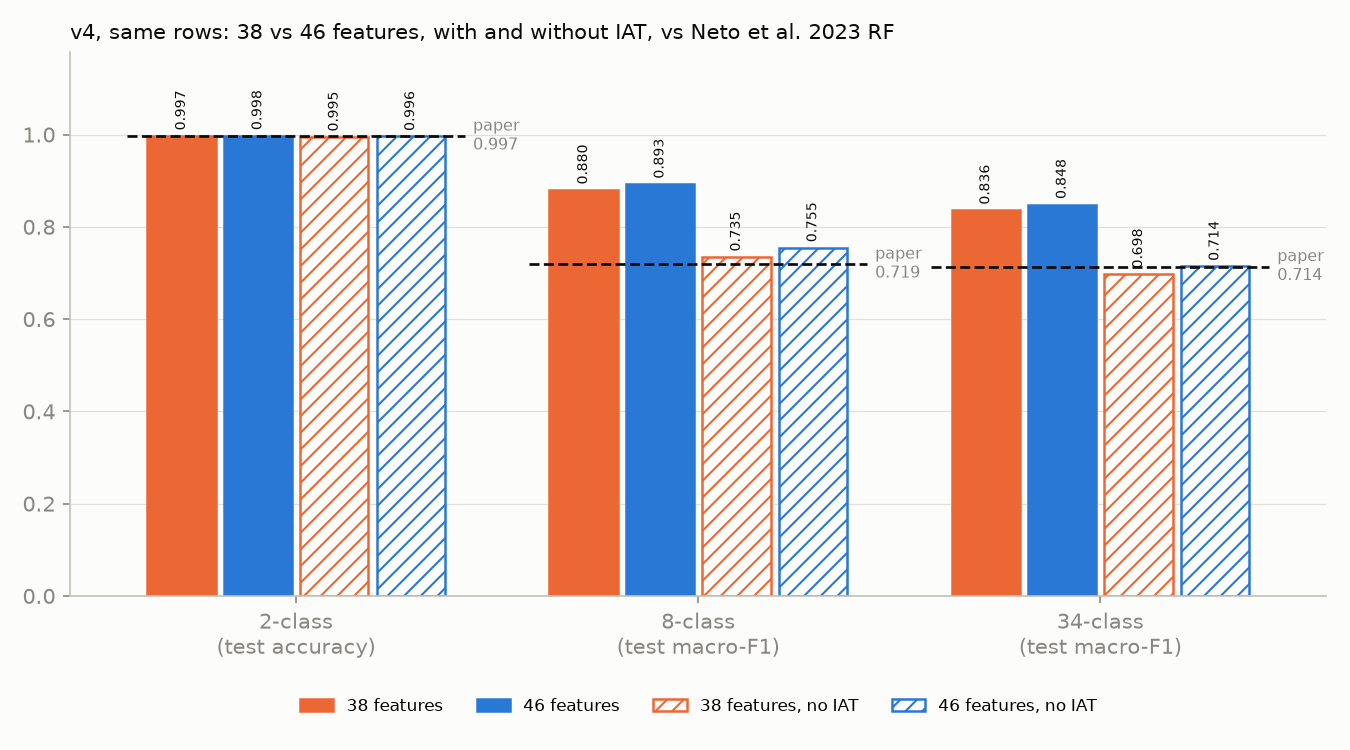
\includegraphics[width=\columnwidth]{fig_v4_ablation.png}
\caption{v4 ablation on the same rows (judged metric per task). Dashed line: Neto et al.~\cite{neto2023ciciot}. Source: \texttt{results/v4\_46feat/summary.json}.}
\label{fig:v4}
\end{figure}

\begin{table*}[!t]
\centering
\caption{Multi-seed results on the full release. Std is the population std over seeds; BEST rows from results/{task}\_class/BEST/multi\_seed\_results.json, others computed from the per-seed JSONs.}\label{tab:multiseed}
\scriptsize
\setlength{\tabcolsep}{3pt}
\begin{tabular}{llp{1.6cm}cc}
\toprule
\textbf{Task} & \textbf{Model} & \textbf{Seeds} & \textbf{Test acc (mean $\pm$ std)} & \textbf{Test mF1 (mean $\pm$ std)} \\
\midrule
2-class & lightgbm\_cfg2 & 42, 123, 456 & 0.9938 $\pm$ 0.000003 & 0.9328 $\pm$ 0.000030 \\
8-class & xgboost\_cfg3\_weighted & 42, 123, 456 & 0.8408 $\pm$ 0.000060 & 0.7317 $\pm$ 0.000056 \\
34-class & xgboost\_balanced\_p050 & 42, 123, 456 & 0.7945 $\pm$ 0.000073 & 0.6434 $\pm$ 0.000157 \\
34-class & hierarchical 8$\rightarrow$34 (hard) & 1, 2, 42 & 0.7714 $\pm$ 0.000051 & 0.6352 $\pm$ 0.000102 \\
2-class & CatBoost c1, no weights & 1, 2, 42 & 0.9927 $\pm$ 0.000045 & 0.9223 $\pm$ 0.000673 \\
34-class & CatBoost c1, no weights & 1, 2, 42 & 0.7749 $\pm$ 0.000054 & 0.5408 $\pm$ 0.001091 \\
\bottomrule
\end{tabular}
\end{table*}

\begin{table*}[!t]
\centering
\caption{Post-hoc methods on the full release (threshold tuning A1, calibration A2, ensembles and stacking A3). The method is chosen by validation macro-F1 only.}\label{tab:posthoc}
\scriptsize
\setlength{\tabcolsep}{3pt}
\begin{tabular}{llp{5.2cm}rrr}
\toprule
\textbf{Ver} & \textbf{Task} & \textbf{Method} & \textbf{Val mF1 (selection)} & \textbf{Test acc} & \textbf{Test mF1} \\
\midrule
v2 & 2 & LightGBM cfg2 + threshold 0.49 & n/a & 0.9937 & 0.9324 \\
v2 & 2 & Soft-vote ensemble (3 models) & n/a & 0.9938 & 0.9332 \\
v3 & 2 & baseline & 0.9323 & 0.9938 & 0.9328 \\
v3 & 2 & A1\_threshold & 0.9328 & 0.9937 & 0.9333 \\
v3 & 2 & A2\_isotonic & 0.9315 & 0.9938 & 0.9329 \\
v3 & 2 & A2\_sigmoid & 0.9253 & 0.9934 & 0.9257 \\
v3 & 2 & A3\_soft & 0.9316 & 0.9937 & 0.9322 \\
v3 & 2 & A3\_weighted & 0.9316 & 0.9937 & 0.9322 \\
v3 & 2 & A3\_weighted+A1 & 0.9320 & 0.9936 & 0.9328 \\
v3 & 2 & A3\_stack & 0.9325 & 0.9938 & 0.9334 \\
v3 & 2 & A3\_stack+A1 (selected by val) & 0.9332 & 0.9937 & 0.9339 \\
v3 & 34 & baseline & 0.6412 & 0.7946 & 0.6429 \\
v3 & 34 & A1\_threshold (selected by val) & 0.6431 & 0.7895 & 0.6452 \\
v3 & 34 & A2\_isotonic & 0.6361 & 0.7980 & 0.6380 \\
v3 & 34 & A2\_sigmoid & 0.6369 & 0.7980 & 0.6386 \\
v3 & 34 & A3\_soft & 0.6394 & 0.7955 & 0.6416 \\
v3 & 34 & A3\_weighted & 0.6402 & 0.7953 & 0.6426 \\
v3 & 34 & A3\_weighted+A1 & 0.6423 & 0.7888 & 0.6461 \\
v3 & 34 & A3\_stack & 0.6367 & 0.7981 & 0.6398 \\
v3 & 34 & A3\_stack+A1 & 0.6423 & 0.7901 & 0.6480 \\
\bottomrule
\end{tabular}
\end{table*}


\begin{figure}[!t]
\centering
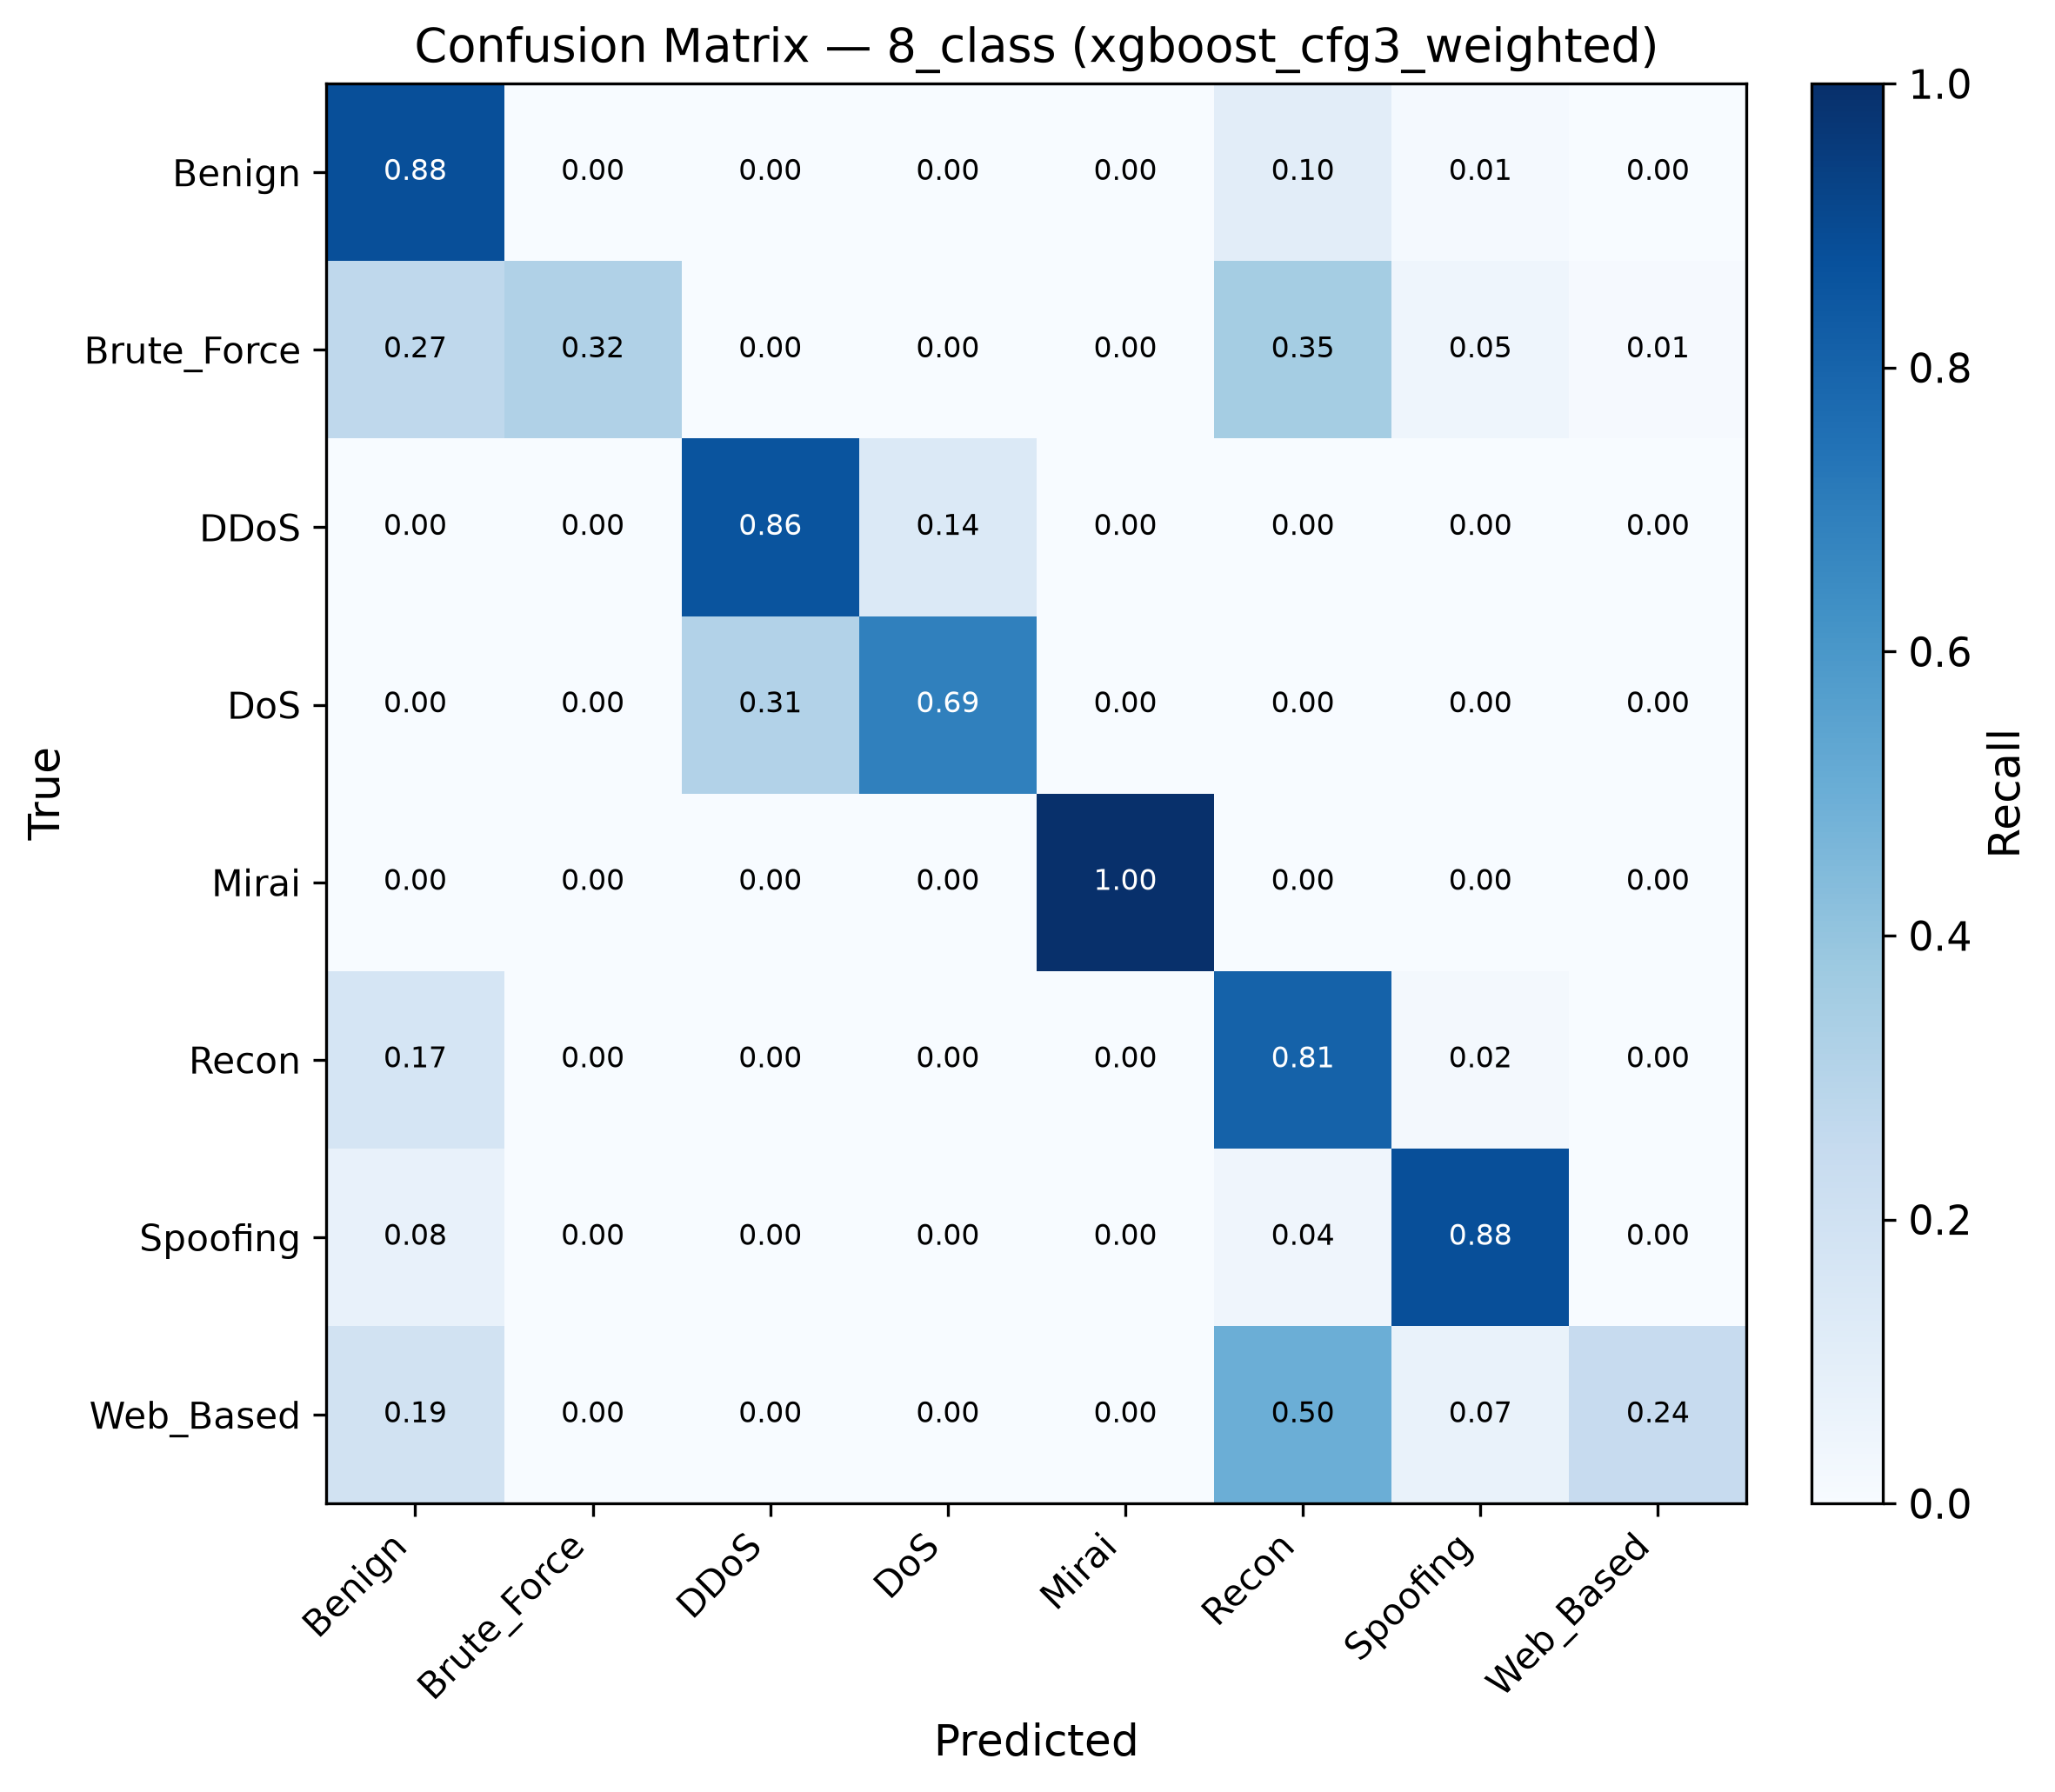
\includegraphics[width=0.85\columnwidth]{fig_cm8_full.png}
\caption{8-class confusion matrix (row-normalised) of the best full-release model, XGBoost cfg3\_weighted.
Source: \texttt{results/8\_class/xgboost\_cfg3\_weighted/results.json}.}
\label{fig:cm8}
\end{figure}

\begin{figure}[!t]
\centering
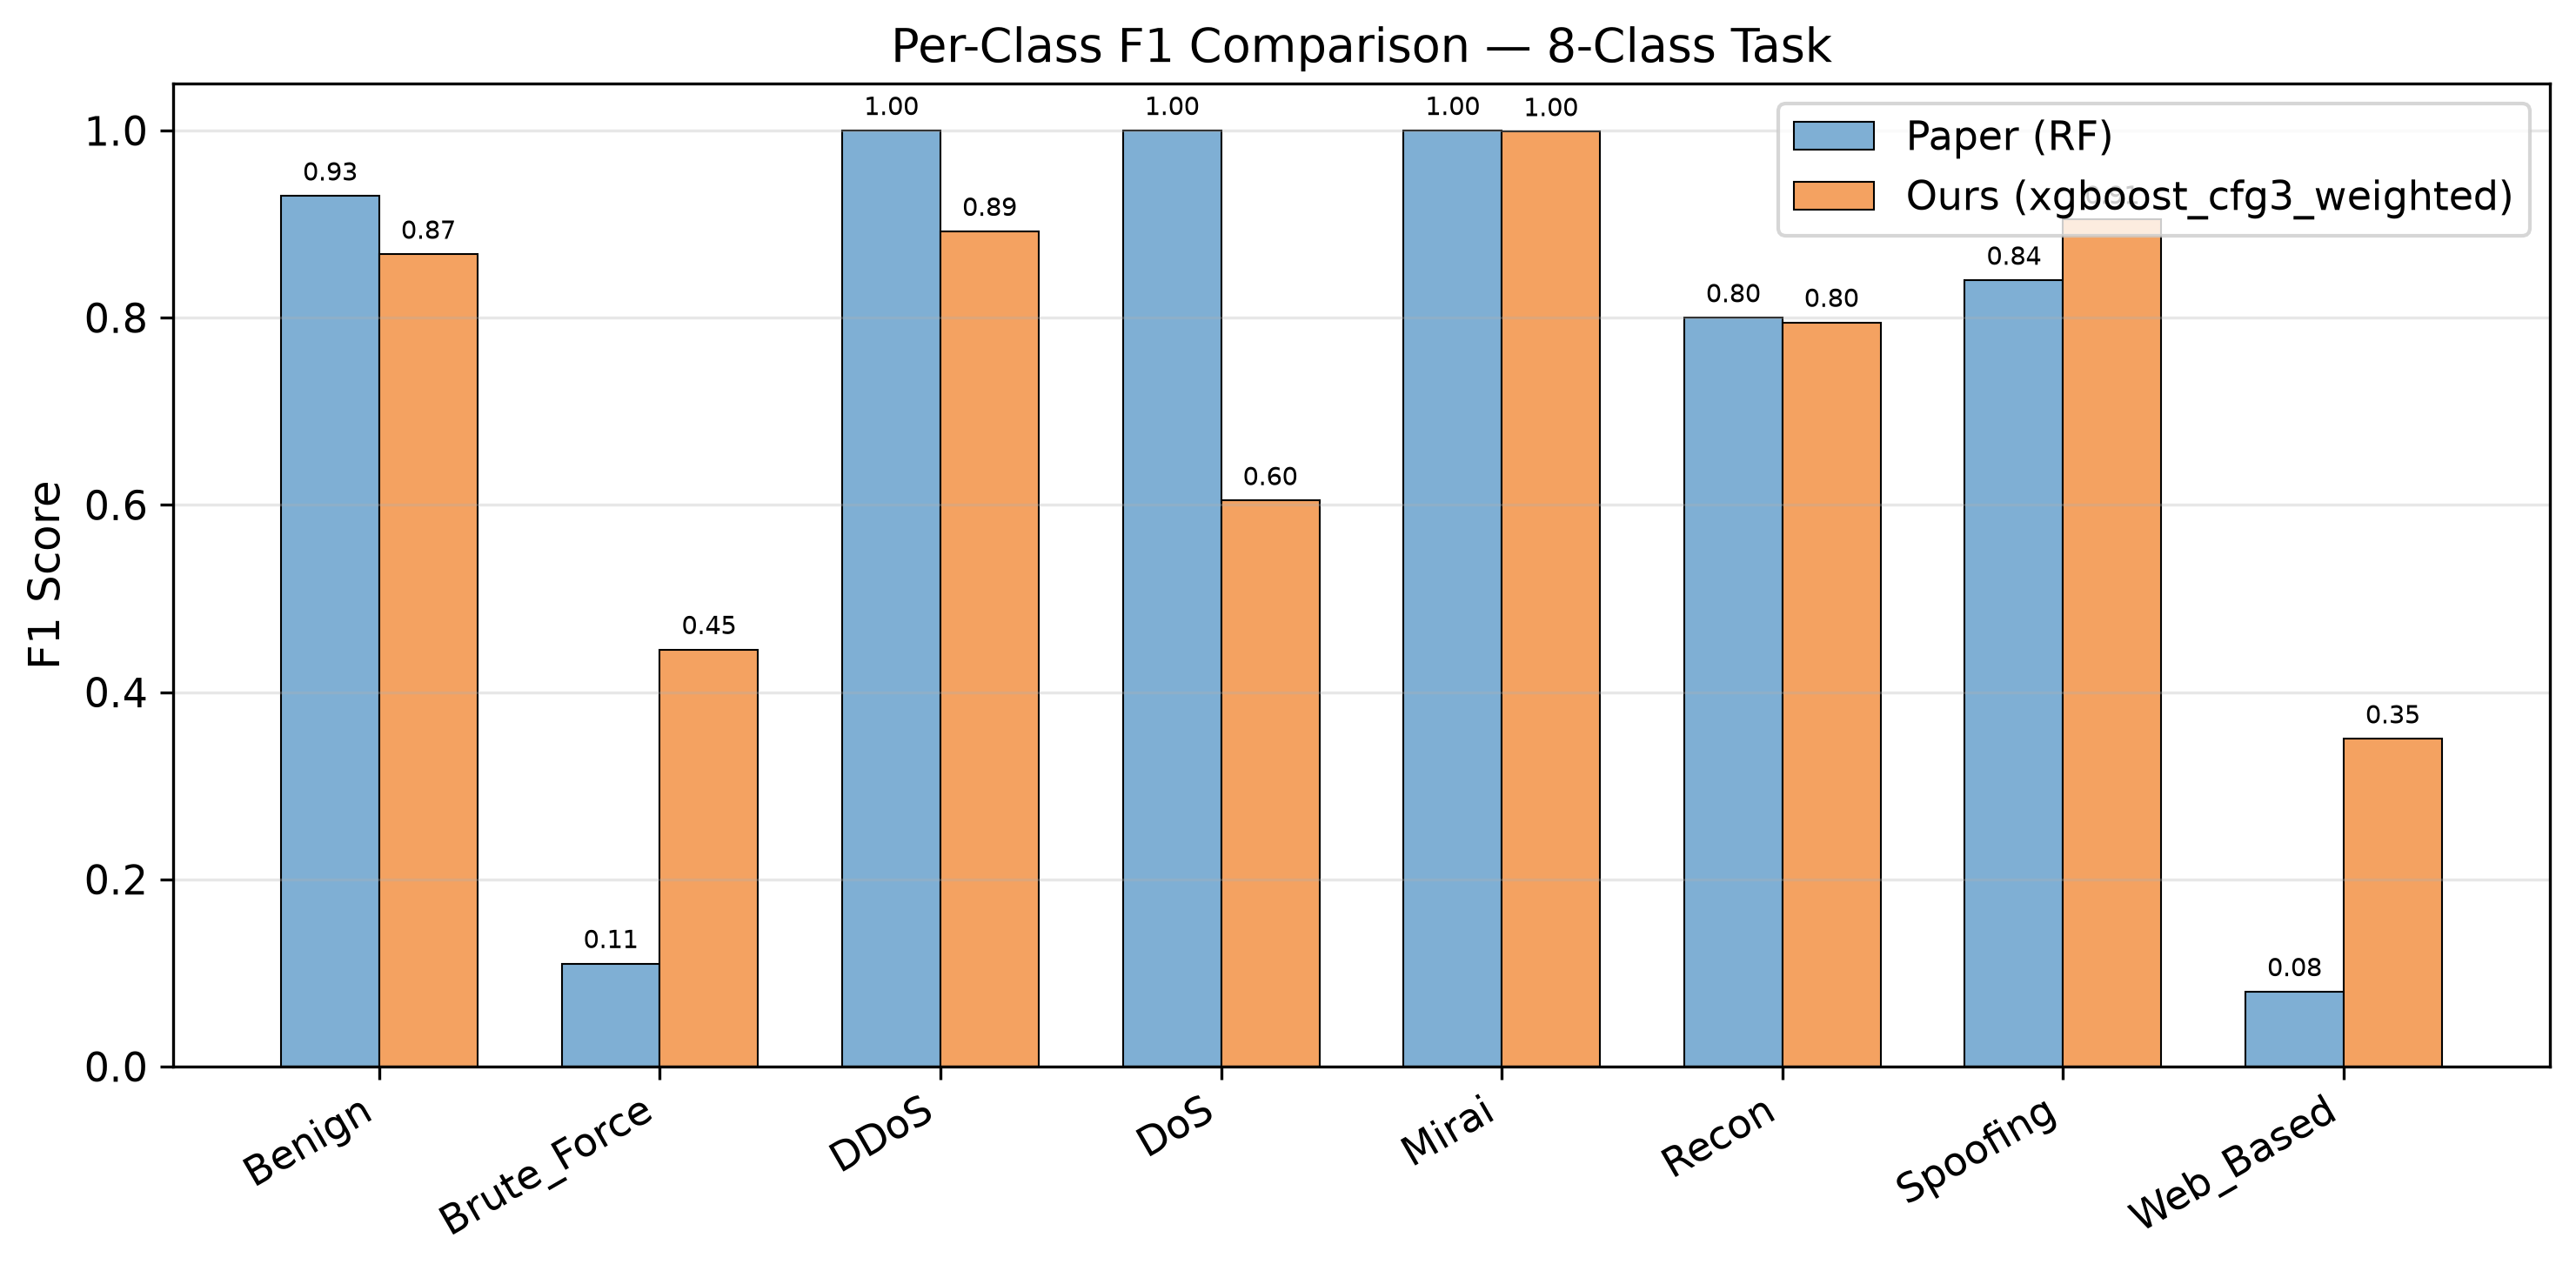
\includegraphics[width=\columnwidth]{fig_perclass_f1_8.png}
\caption{Per-class test F1, 8-class, full release. Brute\_Force, DoS and Web\_Based are the weak classes.
Source: \texttt{results/8\_class/*/results.json}.}
\label{fig:pcf1}
\end{figure}

\begin{figure*}[!t]
\centering
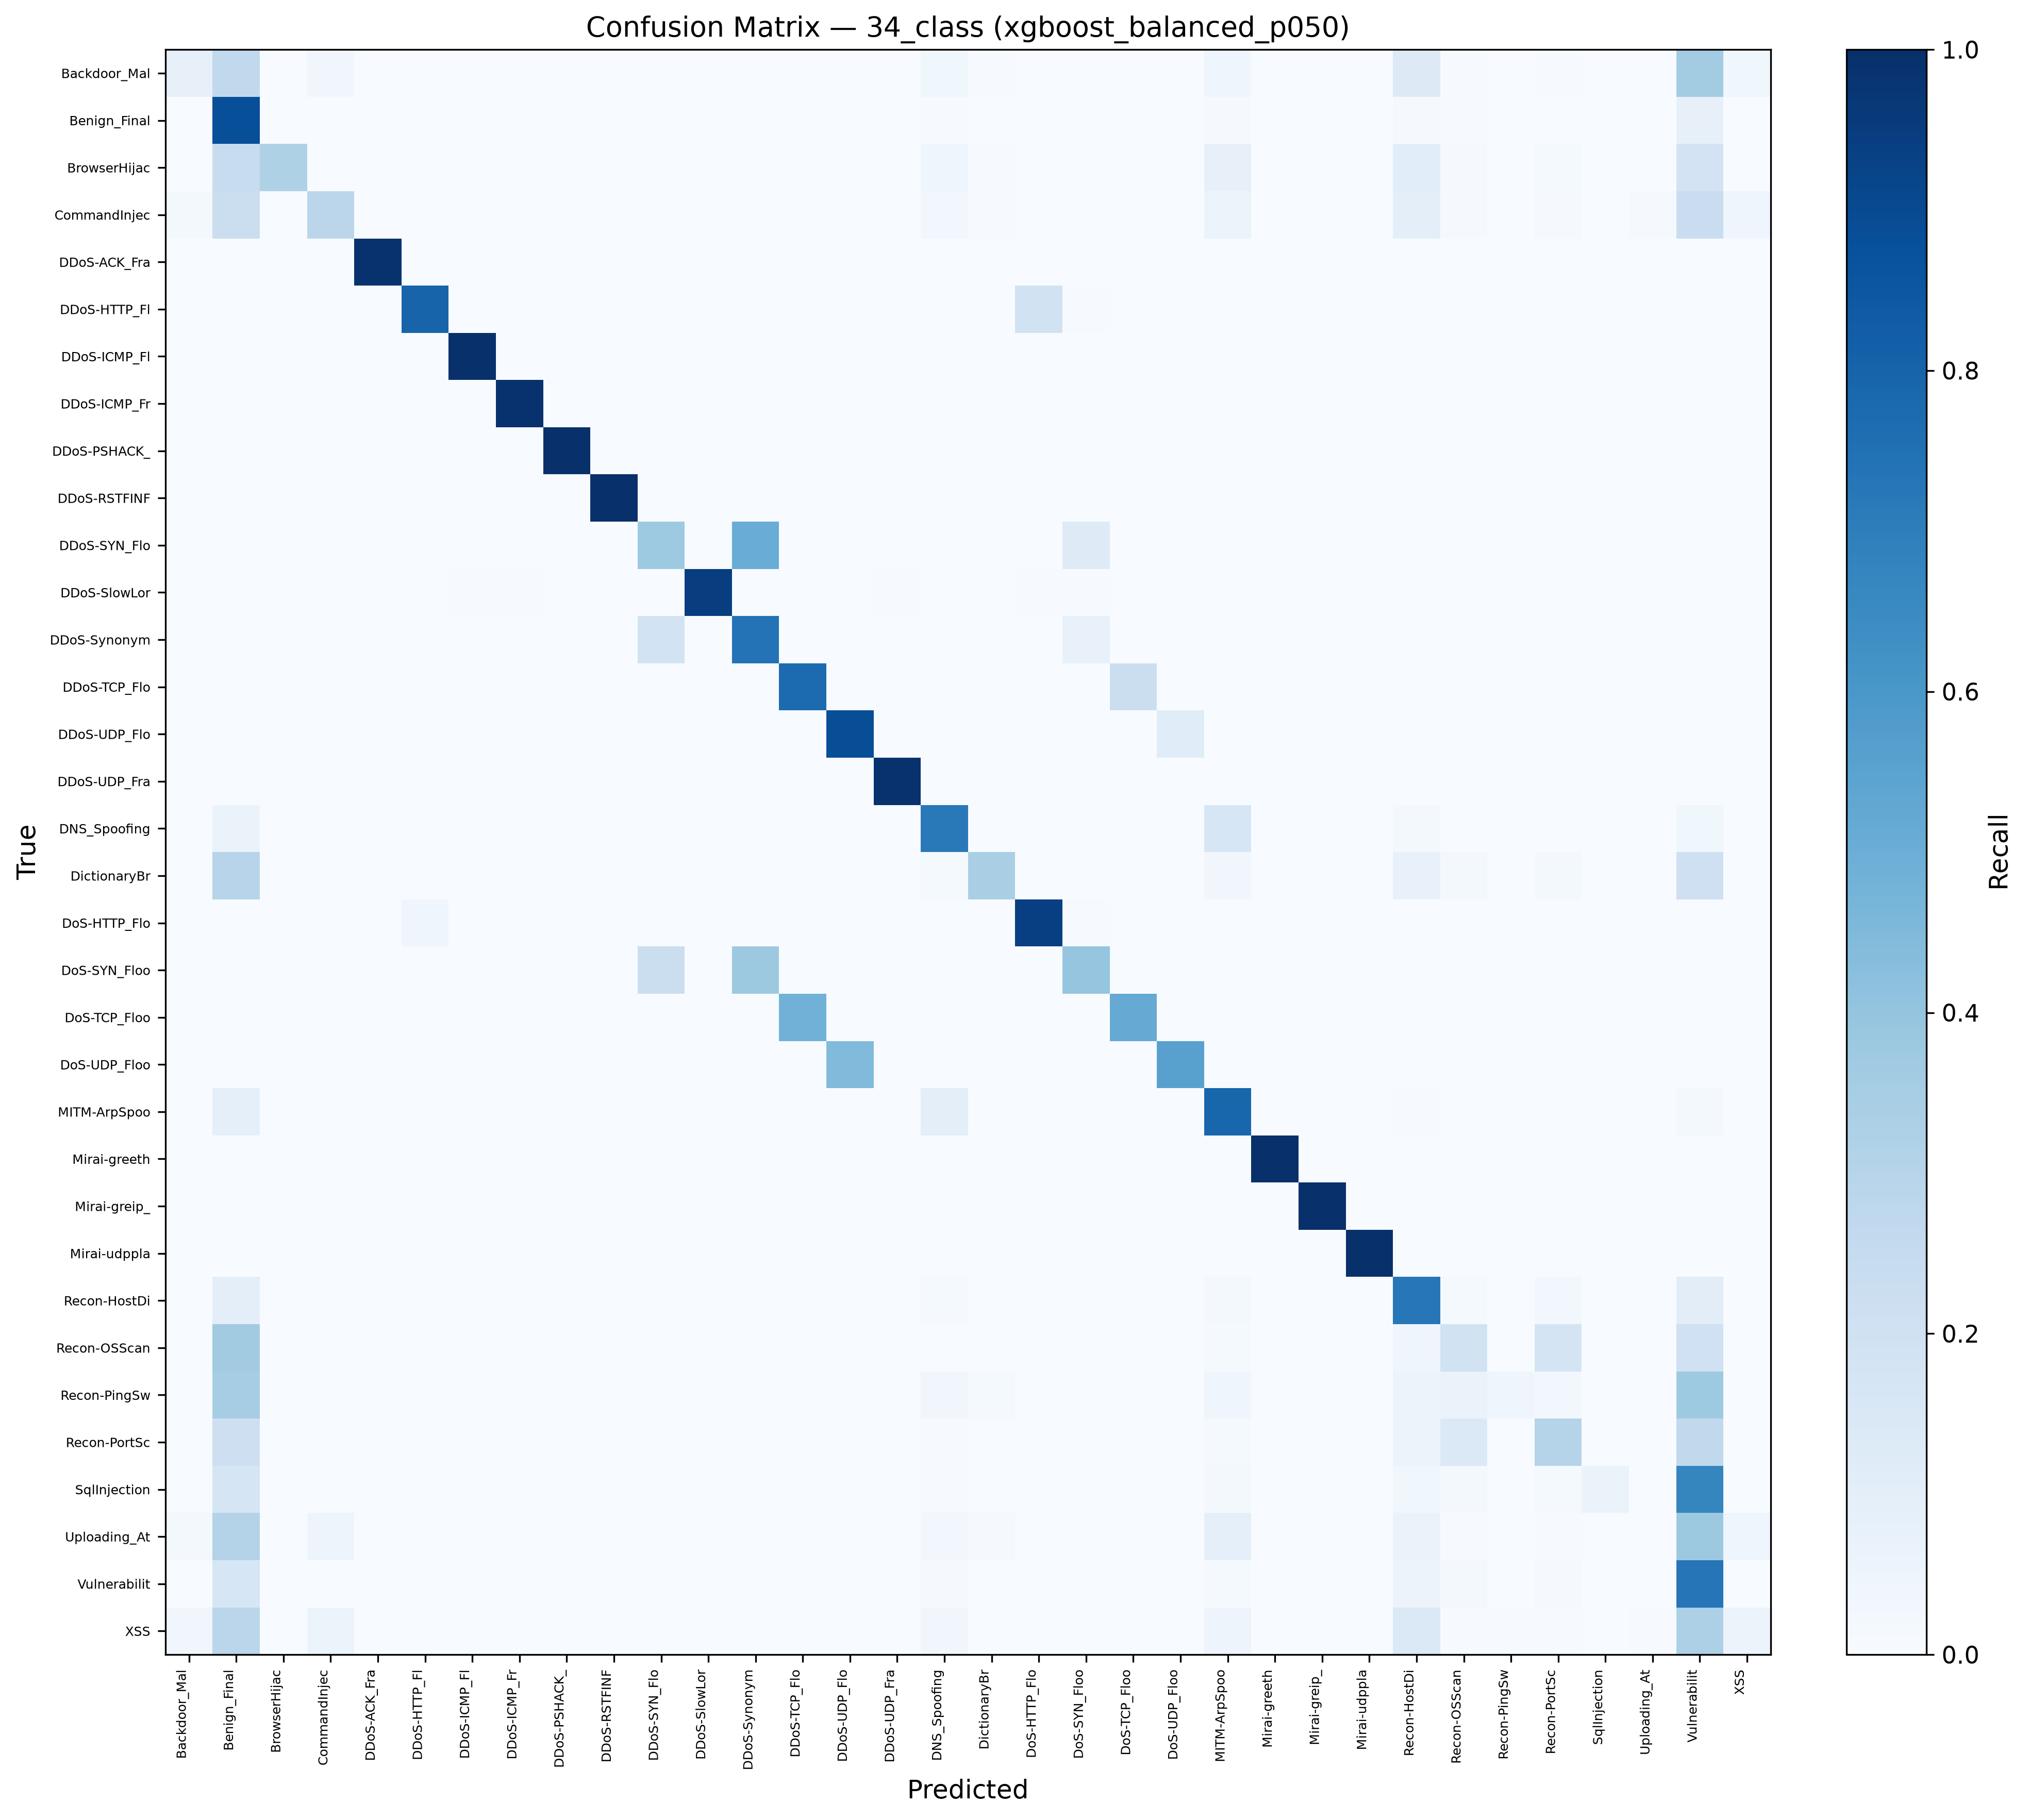
\includegraphics[width=0.62\textwidth]{fig_cm34_full.png}
\caption{34-class confusion matrix (row-normalised) of the best full-release single model. Source:
\texttt{results/34\_class/xgboost\_balanced\_p050/results.json}.}
\label{fig:cm34}
\end{figure*}

%=====================================================================
\section{Analysis and Novelty}
Table~\ref{tab:novelty} summarises the analyses and their evidence files.
\begin{table*}[!t]
\centering
\caption{Summary of the analyses N1-N6 with their evidence files.}\label{tab:novelty}
\scriptsize
\setlength{\tabcolsep}{3pt}
\begin{tabular}{lp{4.2cm}p{3.2cm}p{5.4cm}}
\toprule
\textbf{Analysis} & \textbf{Measure} & \textbf{Value} & \textbf{Evidence (JSON)} \\
\midrule
N1 twins & test rows with an exact train twin & 59.05\% (full) / 5.61\% (v4) & results/novelty/N1\_twin\_analysis/results.json; results/v4\_46feat/summary.json \\
N2 protocol ladder & 8-class mF1: paper protocol $\rightarrow$ file-grouped (twin-free) & 0.7308 $\rightarrow$ 0.4454 (0.4557) & results/novelty/N2\_protocol\_ladder/results.json \\
N3 DoS vs DDoS & share of 8-class test errors (full / v4 no-IAT) & 95.18\% / 92.82\% & results/novelty/v3/dos\_ddos.json; results/v4\_46feat/summary.json \\
N3 merge & 8-class acc $\rightarrow$ 7-class (DoS+DDoS merged) acc & 0.8410 $\rightarrow$ 0.9923 & results/novelty/v3/dos\_ddos.json \\
N4 IAT & IAT-only depth-8 tree, 8-class val acc (majority baseline) & 0.9905 (0.7278) & results/v4\_46feat/iat\_probe.json \\
N5 window & capture-window classifier accuracy & 99.9997\% & results/novelty/N5\_window\_size/results.json \\
N6 hierarchical & 34-class test mF1, hierarchical (3 seeds) vs flat & 0.6352 vs 0.6429 & results/novelty/v3/hierarchical\_s*.json \\
\bottomrule
\end{tabular}
\end{table*}


\textbf{N1 -- twin leakage.} Under the shuffled 75/5/20 split, \nOneTwin{} of full-release test rows are exact
duplicates (``twins'') of a training row: \nOneDDoS{} for DDoS but only \nOneBenign{} for benign
(Table~\ref{tab:n1}, Fig.~\ref{fig:twins}). On twin rows the 8-class macro-F1 is \nOneTwinMf{}, compared with
\nOneNonTwinMf{} on non-twin rows. In the v4 subset only \vfTwin{} of test rows have a twin (\vfDup{} of all
rows are duplicates), so twins do not explain the v4 scores.

\begin{table}[!t]
\centering
\caption{N1: twin rate per class on the full release (75/5/20 split).}\label{tab:n1}
\scriptsize
\setlength{\tabcolsep}{3pt}
\begin{tabular}{lr}
\toprule
\textbf{8-class label} & \textbf{Test rows with exact train twin} \\
\midrule
DDoS & 67.61\% \\
DoS & 55.52\% \\
Mirai & 9.26\% \\
Spoofing & 7.06\% \\
Recon & 1.33\% \\
Web\_Based & 0.79\% \\
Benign & 0.54\% \\
Brute\_Force & 0.23\% \\
\bottomrule
\end{tabular}
\end{table}


\begin{figure}[!t]
\centering
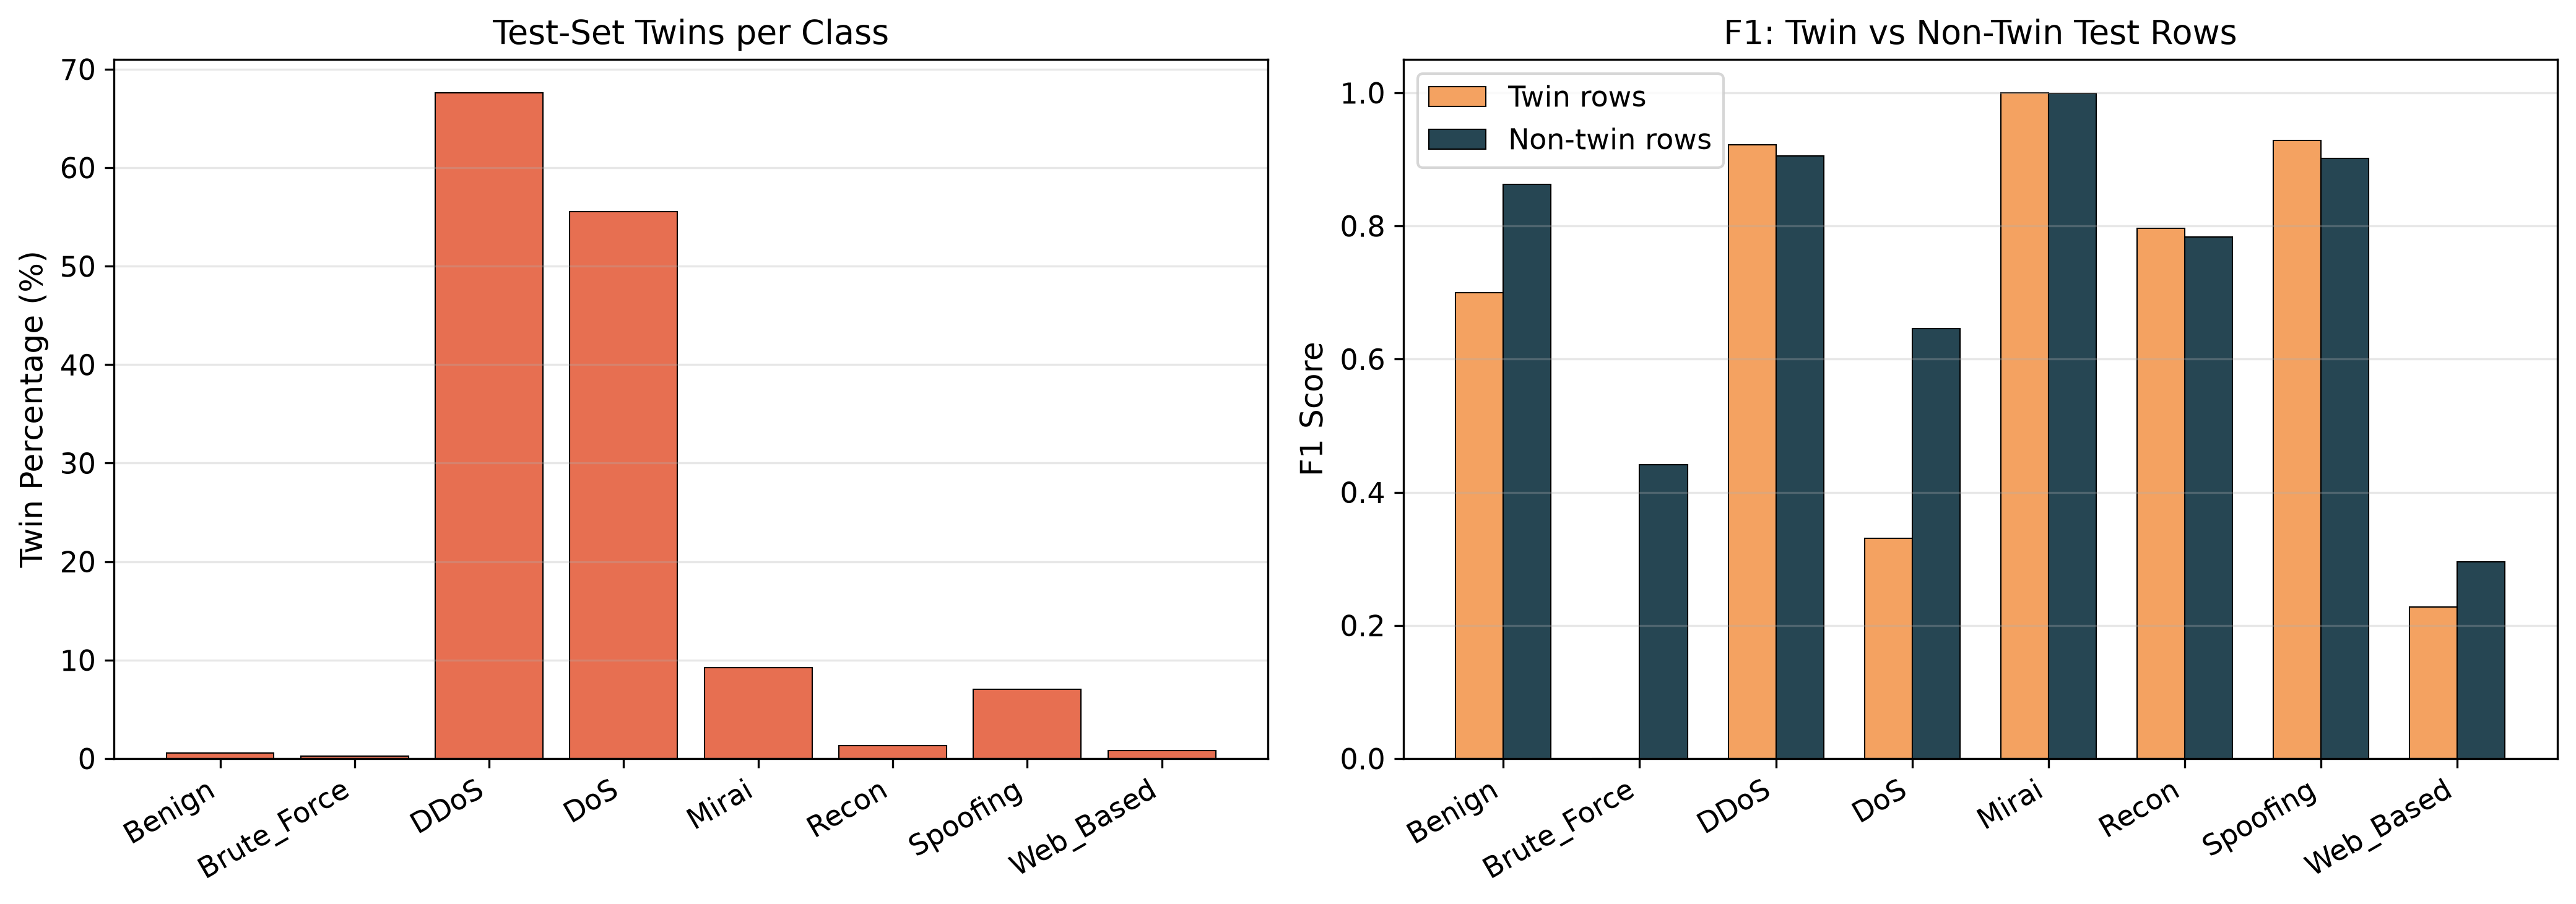
\includegraphics[width=\columnwidth]{fig_twins.png}
\caption{N1: twin share per class and F1 on twin vs non-twin test rows (full release). Source:
\texttt{results/novelty/N1\_twin\_analysis/results.json}.}
\label{fig:twins}
\end{figure}

\textbf{N2 -- protocol ladder.} Keeping the model fixed (8-class XGBoost balanced\_deep), we tighten the
protocol step by step (Table~\ref{tab:n2}, Fig.~\ref{fig:ladder}). De-duplication alone (removing
\nTwoDedupPct{} of rows) barely changes macro-F1 (\nTwoAMf{} $\rightarrow$ \nTwoBMf{}). Grouping by source
file, so that no capture file contributes to both train and test, drops it to \nTwoCMf{} (\nTwoDMf{} when
also twin-free), a fall of \nTwoDrop{} from the paper protocol to the strictest one.

\begin{table}[!t]
\centering
\caption{N2: protocol ladder on the full release.}\label{tab:n2}
\scriptsize
\setlength{\tabcolsep}{3pt}
\begin{tabular}{p{4.6cm}rr}
\toprule
\textbf{Protocol (8-class, XGBoost balanced\_deep)} & \textbf{Test acc} & \textbf{Test mF1} \\
\midrule
(a) paper protocol: shuffled rows, no de-dup & 0.8415 & 0.7308 \\
(b) + de-duplication & 0.8572 & 0.7297 \\
(c) file-grouped split & 0.7455 & 0.4454 \\
(d) file-grouped + twin-free & 0.7217 & 0.4557 \\
\bottomrule
\end{tabular}
\end{table}


\begin{figure}[!t]
\centering
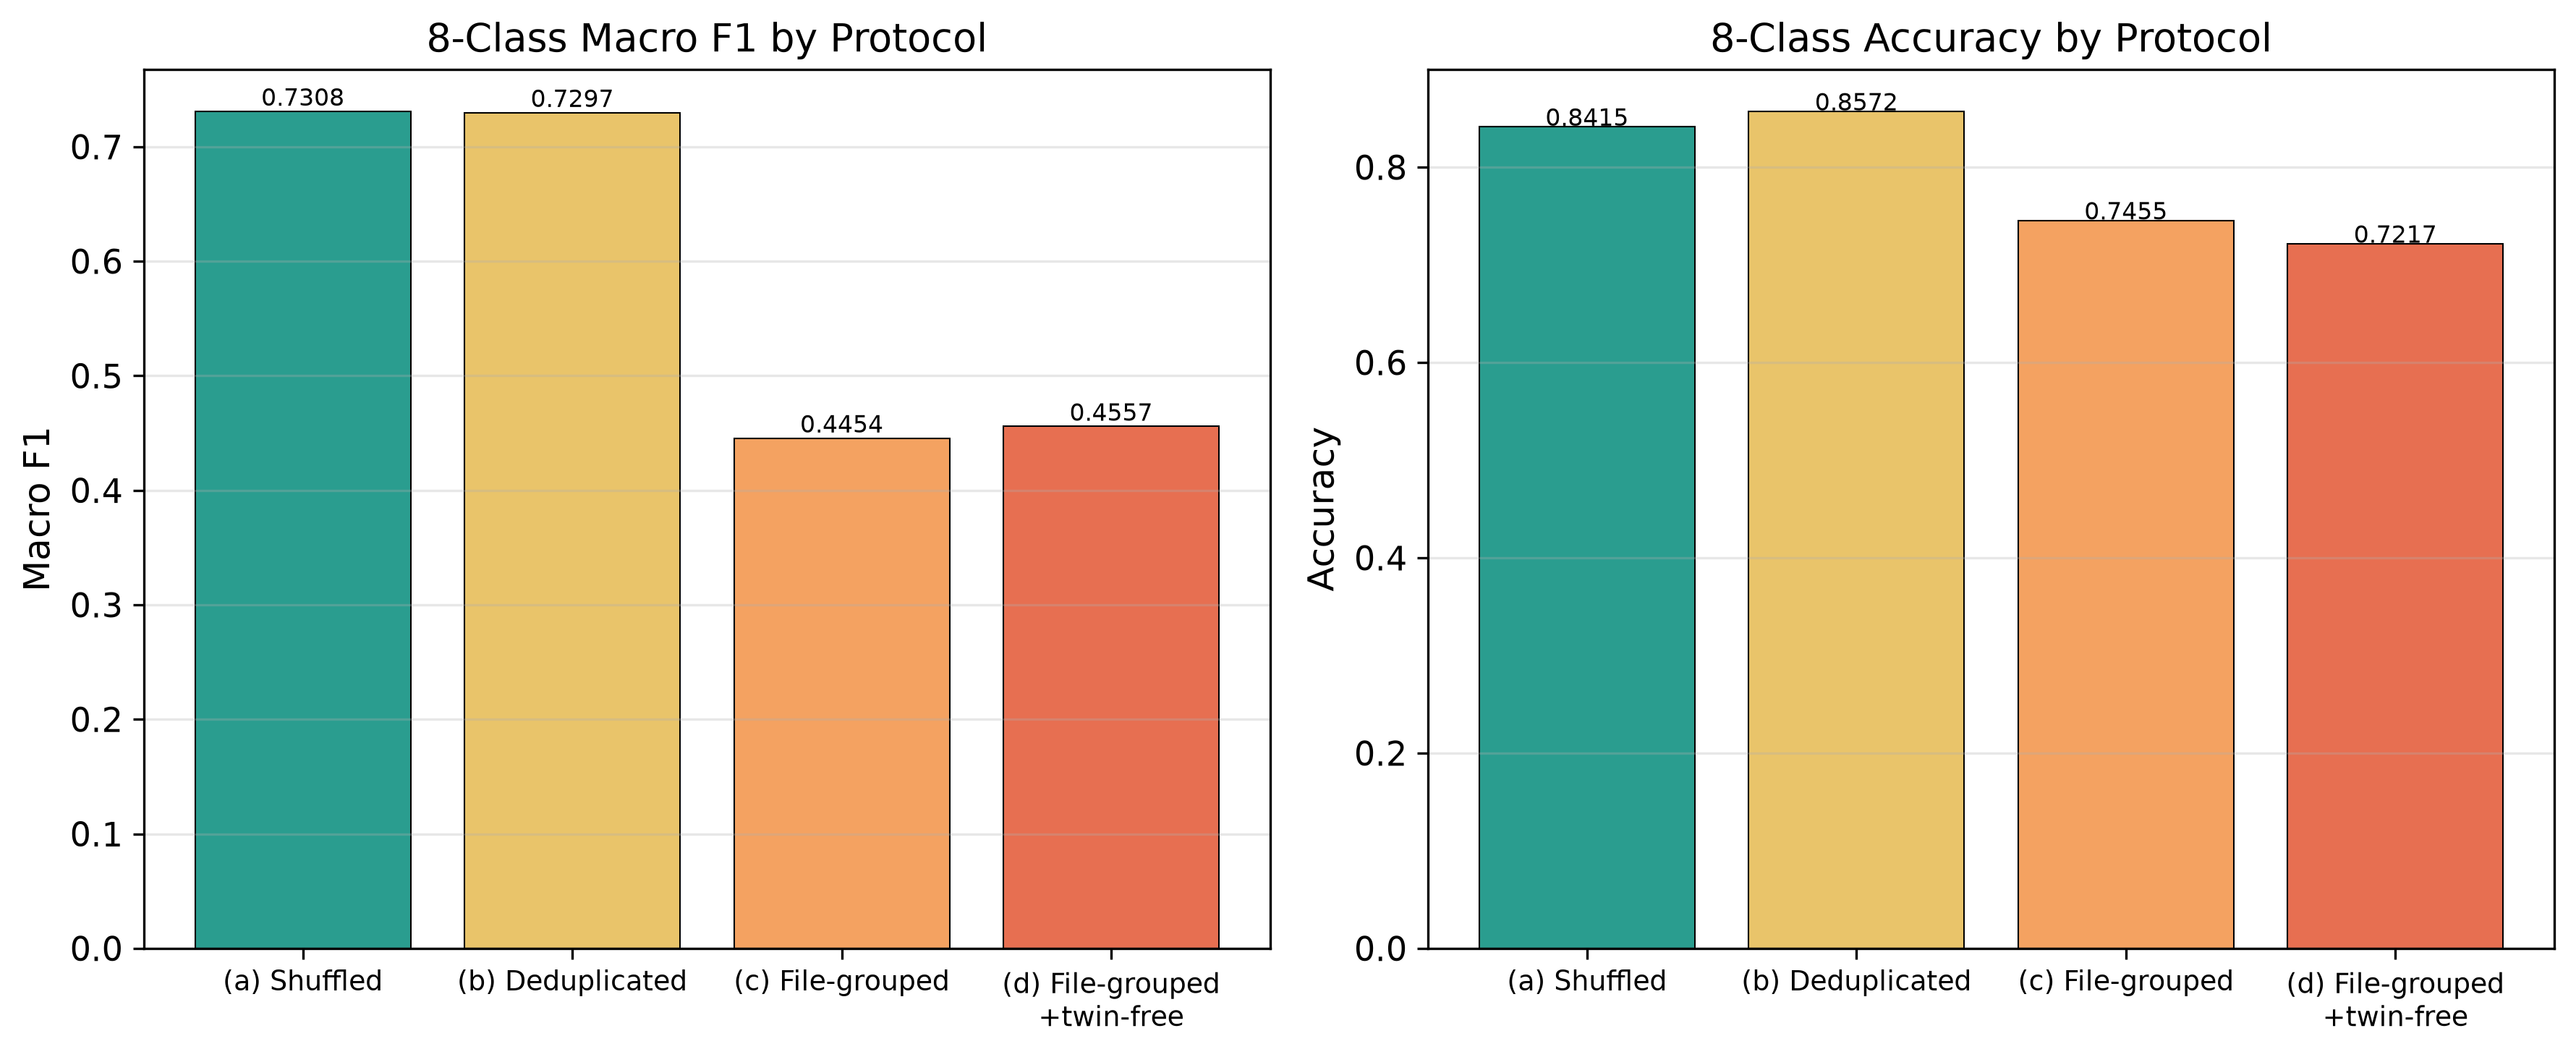
\includegraphics[width=\columnwidth]{fig_protocol_ladder.png}
\caption{N2: 8-class macro-F1 and accuracy under four protocols. Source:
\texttt{results/novelty/N2\_protocol\_ladder/results.json}.}
\label{fig:ladder}
\end{figure}

\textbf{N3 -- DoS vs DDoS.} On the full release, DoS$\leftrightarrow$DDoS confusions are \nThreeShare{} of all
8-class test errors. Re-scoring the \emph{same} predictions with DoS and DDoS merged into one class raises
accuracy from \nThreeEightAcc{} to \nThreeFloodAcc{} (macro-F1 \nThreeEightMf{} $\rightarrow$ \nThreeFloodMf{};
Fig.~\ref{fig:merge}). A binary DoS-vs-DDoS model falls from \nThreeBinPaper{} to \nThreeBinGroup{} accuracy
under a file-grouped split. Single-source and distributed floods look the same per flow; the difference is in
the aggregate traffic. In v4 the confusion almost disappears when IAT is used (\vfDdWith{} errors,
\vfDdWithShare{}) and returns without IAT (\vfDdNo{} errors, \vfDdNoShare{}). The 8 paper-only features do not
remove it (38 features without IAT: \vfDdNoA{}).

\begin{figure}[!t]
\centering
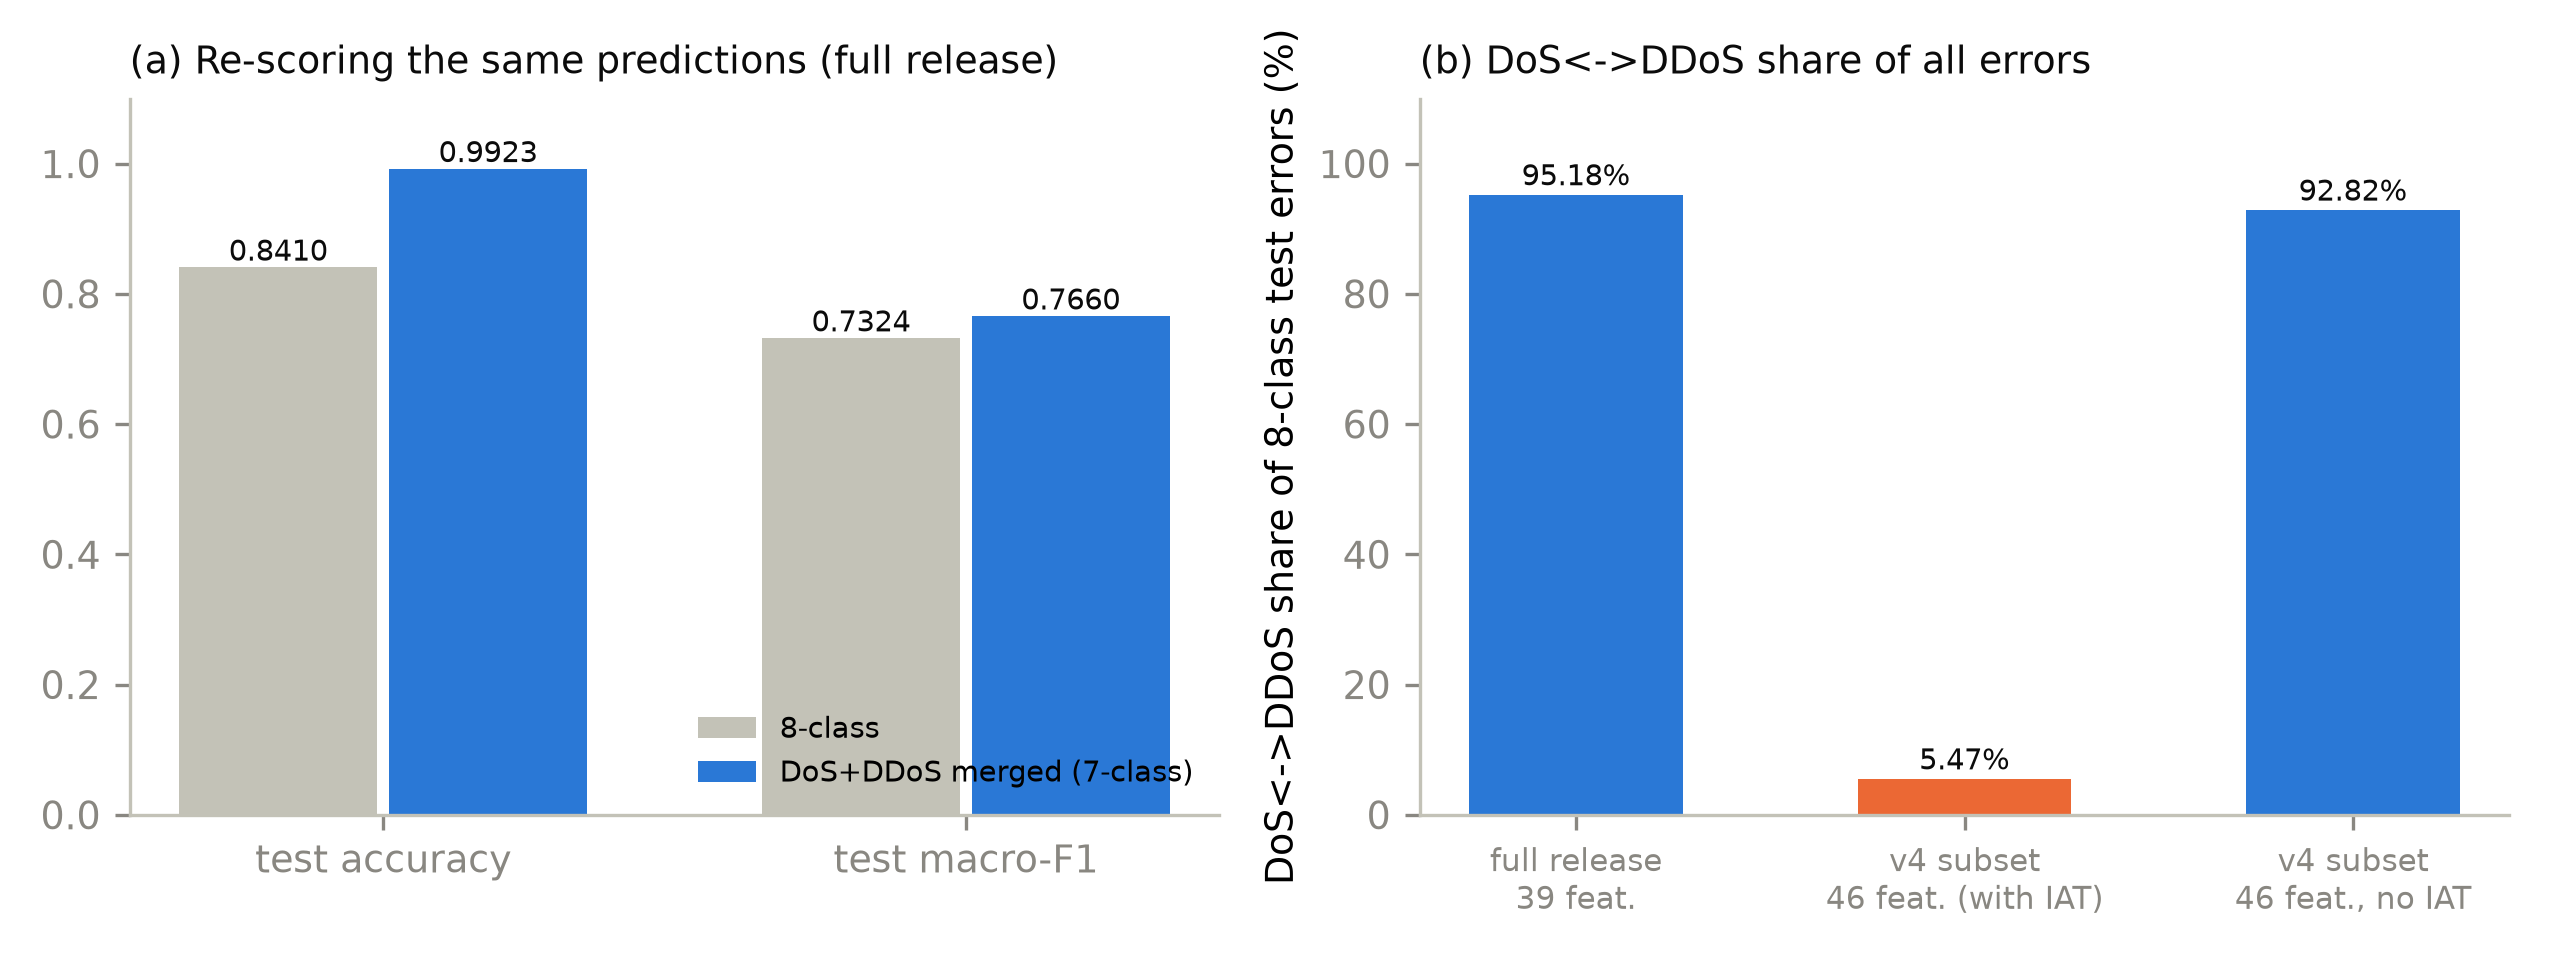
\includegraphics[width=\columnwidth]{fig_dosddos_merge.png}
\caption{N3: (a) merging DoS and DDoS on the same predictions; (b) DoS$\leftrightarrow$DDoS share of 8-class
test errors. Sources: \texttt{results/novelty/v3/dos\_ddos.json}, \texttt{results/v4\_46feat/summary.json}.}
\label{fig:merge}
\end{figure}

\textbf{N4 -- IAT acts as a capture timestamp.}\label{sec:iat} In the v4 subset, the median raw IAT is \iatMedDoSTCP{} for DoS-TCP\_Flood,
\iatMedDDoSICMP{} for DDoS-ICMP\_Flood and \iatMedBenign{} for benign traffic, and each attack class occupies its
own narrow band (Table~\ref{tab:iat}, Fig.~\ref{fig:iat}). Values of this size do not fit the
paper's description of IAT as ``the time difference with the previous packet''~\cite{neto2023ciciot}; they
behave like a capture clock. A depth-8 decision tree on IAT alone reaches \iatAcc{} 8-class validation
accuracy (macro-F1 \iatMf{}; majority class \iatMaj{}). The next-best single feature (\iatSecondName{}) reaches
\iatSecondAcc{}. IAT carries \iatImpEight{} of the gain in the 46-feature 8-class model
(Fig.~\ref{fig:imp}). Without IAT, the 46-feature results fall to \vfDAccTwo{} accuracy (2-class, below the
paper), \vfDMfEight{} macro-F1 (8-class, still above \paperMfEight{}) and \vfDMfThirtyFour{} (34-class, a tie
with \paperMfThirtyFour{}); 8-class accuracy falls from \vfBAccEight{} to \vfDAccEight{}. On the full release,
by contrast, removing TTL and IAT changed 2-class accuracy by only \nFourDrop{} (baseline \nFourBase{}), so
the proxy is specific to this data version.

\begin{table}[!t]
\centering
\caption{N4: per-class IAT quantiles in the Kaggle subset (selected classes; all 34 in results/v4\_46feat/iat\_probe.json).}\label{tab:iat}
\scriptsize
\setlength{\tabcolsep}{3pt}
\begin{tabular}{lrrr}
\toprule
\textbf{Raw label (Kaggle)} & \textbf{IAT 1st pct} & \textbf{IAT median} & \textbf{IAT 99th pct} \\
\midrule
DoS-TCP\_Flood & 8.293e+07 & 8.295e+07 & 8.296e+07 \\
DoS-SYN\_Flood & 8.297e+07 & 8.298e+07 & 8.299e+07 \\
DoS-UDP\_Flood & 8.3e+07 & 8.301e+07 & 8.303e+07 \\
DDoS-TCP\_Flood & 8.303e+07 & 8.307e+07 & 8.308e+07 \\
DDoS-SYN\_Flood & 8.308e+07 & 8.309e+07 & 8.35e+07 \\
DDoS-ICMP\_Flood & 8.312e+07 & 8.313e+07 & 8.348e+07 \\
Mirai-greeth\_flood & 8.368e+07 & 8.368e+07 & 8.37e+07 \\
BenignTraffic & 7.46e-05 & 1.665e+08 & 1.665e+08 \\
DNS\_Spoofing & 3.6e-06 & 1.669e+08 & 1.669e+08 \\
XSS & 0.0001907 & 1.676e+08 & 1.676e+08 \\
\bottomrule
\end{tabular}
\end{table}


\begin{figure*}[!t]
\centering
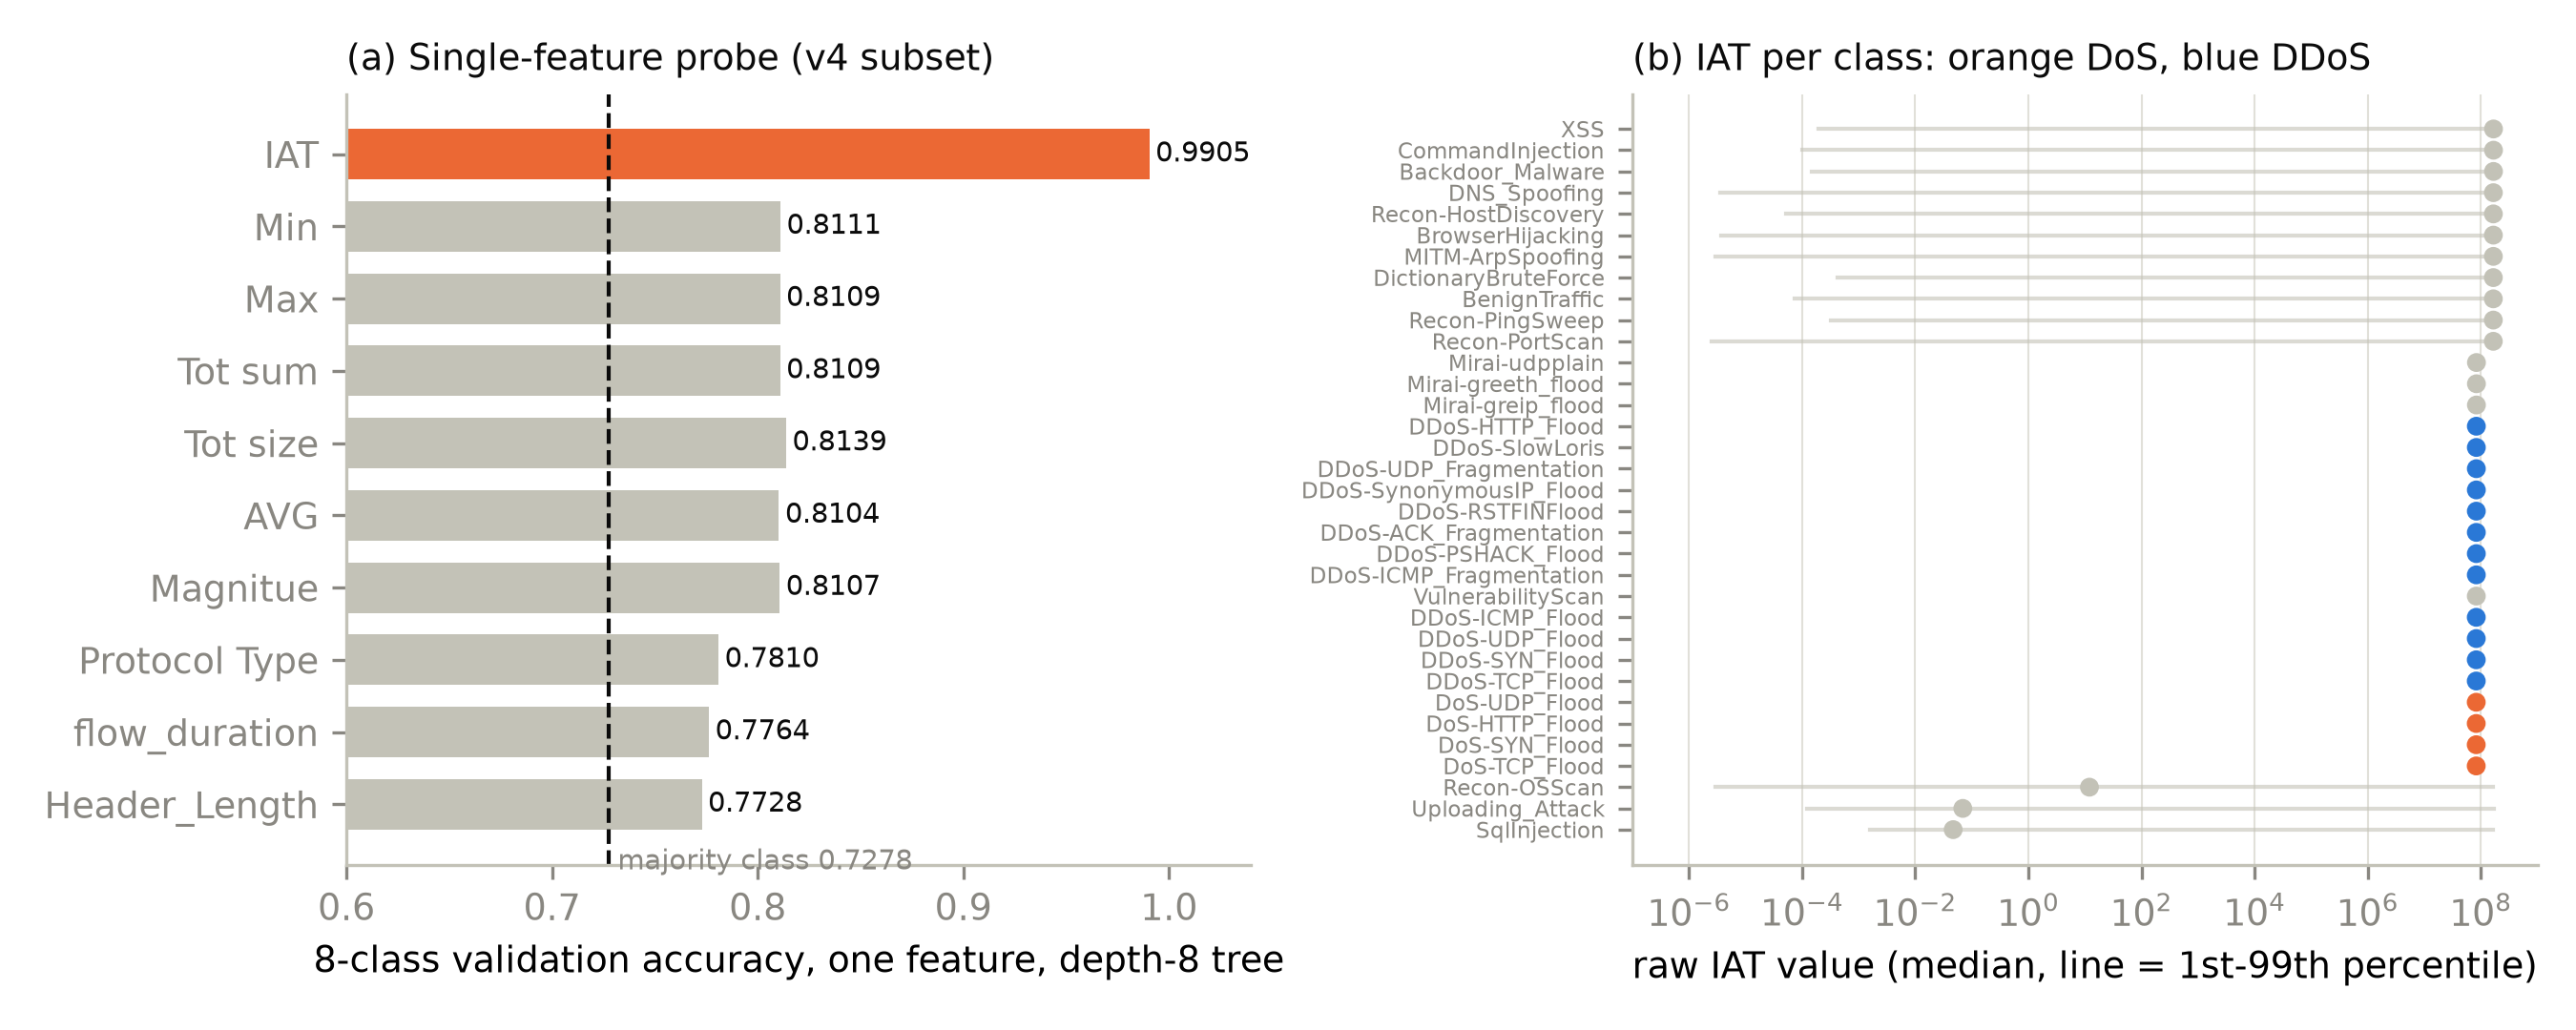
\includegraphics[width=0.9\textwidth]{fig_iat_probe.png}
\caption{N4: (a) single-feature probe, 8-class validation accuracy of a depth-8 tree per feature; (b)
per-class IAT median and 1st--99th percentile range (log scale). Source:
\texttt{results/v4\_46feat/iat\_probe.json}.}
\label{fig:iat}
\end{figure*}

\begin{figure*}[!t]
\centering
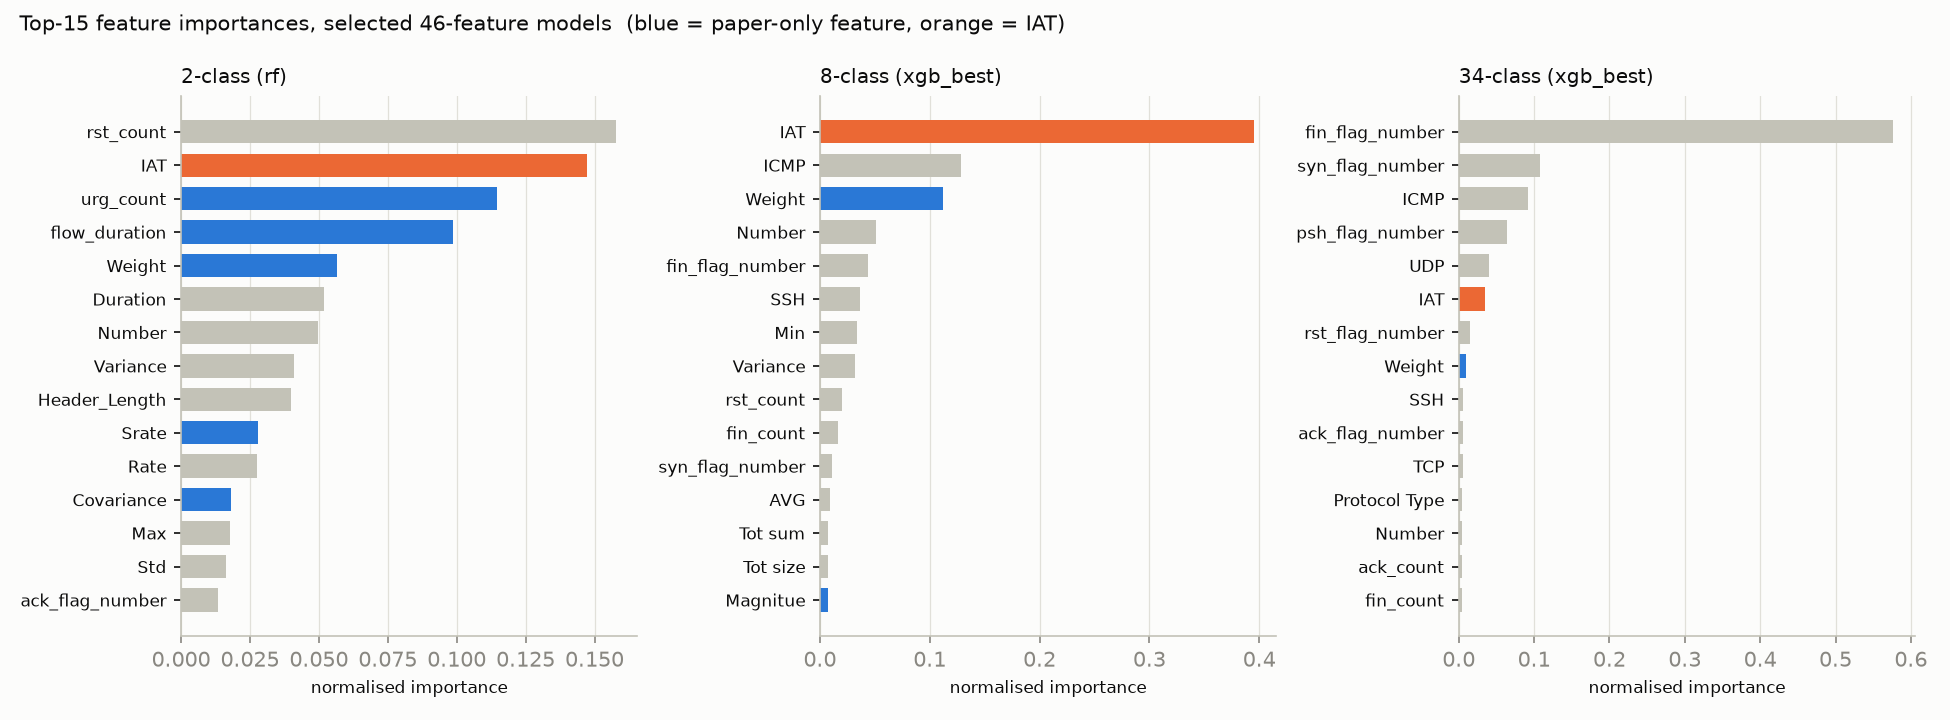
\includegraphics[width=0.95\textwidth]{fig_v4_importance.png}
\caption{Top-15 feature importances of the selected 46-feature models (blue: paper-only features; orange:
IAT). Source: \texttt{results/v4\_46feat/summary.json}.}
\label{fig:imp}
\end{figure*}

\textbf{N5 -- window-size artifact.} The paper averages packets over windows of 10 or 100 packets ``to mitigate
data size discrepancy''~\cite{neto2023ciciot}. A classifier recovers a row's capture window with
\nFiveAcc{} accuracy from its features (top features: Number, Header\_Length, Protocol Type), so
window-level artifacts are visible to any model. Removing the window features changes 8-class macro-F1 by
\nFiveMfChange{}.

\textbf{N6 -- negative results.} The hierarchical 8$\rightarrow$34 classifier reaches a 34-class test
macro-F1 of \hierMf{} $\pm$ \hierMfSd{} over 3 seeds, below the flat XGBoost (\flatMfThirtyFour{};
Fig.~\ref{fig:hier}): subtypes inside a family are easy to separate, and the errors come from the family
level. The best CatBoost GPU run (by validation) gives \cbBestMf{}, and focal reweighting gives \focalMf{}. The
class-weight sweep peaks at power \nSixBestP{} (8-class macro-F1 \nSixBestMf{}).

\begin{figure}[!t]
\centering
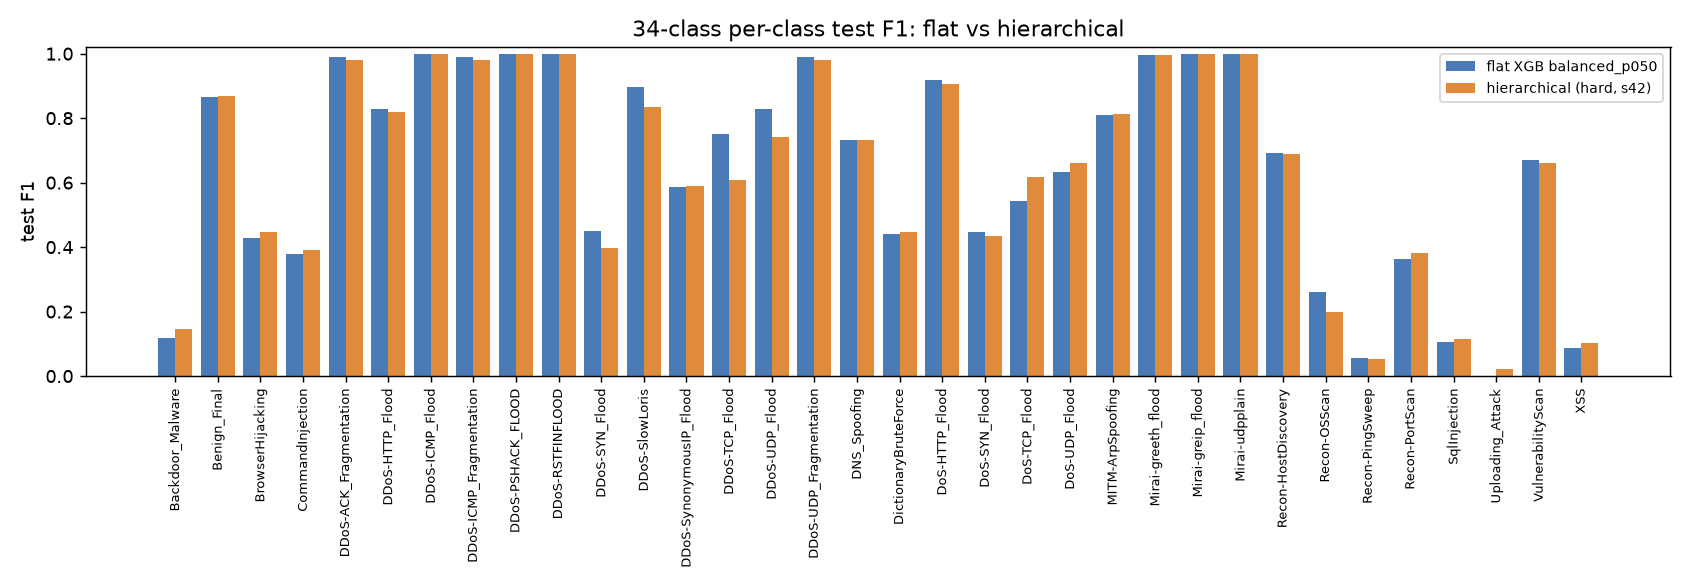
\includegraphics[width=\columnwidth]{fig_hier_f1.png}
\caption{N6: per-class 34-class F1, flat vs hierarchical. Source: \texttt{results/novelty/v3/hierarchical\_s42.json}.}
\label{fig:hier}
\end{figure}

\textbf{N7 -- the benchmark used IAT.} Table~4 of~\cite{neto2023ciciot} (``Features extracted from the network
traffic'') lists 47 features. The list below is quoted from the paper exactly as rendered in the PubMed Central copy,
where three names appear truncated (marked [sic]):
\begin{quote}\footnotesize
\emph{ts, flow duration, Header Length, Protocol Type, Duration, Rate, Srate, Drate, fin flag number, syn
flag number, rst flag number, psh flag numbe [sic], ack flag number, ece flag numbe [sic], cwr flag number, ack count,
syn count, fin count, urg coun [sic], rst count, HTTP, HTTPS, DNS, Telnet, SMTP, SSH, IRC, TCP, UDP, DHCP, ARP,
ICMP, IPv, LLC, Tot sum, Min, Max, AVG, Std, Tot size, IAT, Number, Magnitude, Radius, Covariance,
Variance, Weight} --- from~\cite{neto2023ciciot}, Table~4.
\end{quote}
IAT is described there as ``The time difference with the previous packet'', and the cleaning step states: ``In
our experiments, we only remove the timestamp from the list since it does not illustrate the network
behavior''~\cite{neto2023ciciot}. Only \emph{ts} was dropped, so the paper's models had IAT available. Given N4,
the published 99\% accuracies most likely rely in part on this capture-time proxy. We cannot re-run the
authors' code, so this is an inference from their stated pipeline and our measurements.

%=====================================================================
\section{Intrusion Prevention (IDPS)}
We deploy the best no-IAT 8-class model (XGBoost cfg3\_weighted, 45 features) behind a policy that maps each
class to an action (Table~\ref{tab:policy}). DoS and DDoS share one action because they are the pair the
model confuses most. BLOCK generates an \texttt{iptables} hashlimit rate-limit rule and BLOCK+ALERT a drop
rule. Because CICIoT2023 has no IP addresses, the rules use placeholder sources from 203.0.113.0/24 and are
generated as text, never executed.

\begin{table}[!t]
\centering
\caption{IDPS policy (src/prevention/policy.json).}\label{tab:policy}
\scriptsize
\setlength{\tabcolsep}{3pt}
\begin{tabular}{ll}
\toprule
\textbf{8-class label} & \textbf{Action} \\
\midrule
Benign & ALLOW \\
DDoS & BLOCK \\
DoS & BLOCK \\
Mirai & BLOCK \\
Recon & ALERT \\
Spoofing & BLOCK+ALERT \\
Web\_Based & BLOCK+ALERT \\
Brute\_Force & BLOCK+ALERT \\
\bottomrule
\end{tabular}
\end{table}


We replay \idsRows{} v4 test flows in random order. Plain 8-class accuracy is \idsEightAcc{}, but action
accuracy is \idsActAcc{}: of the \idsErr{} class errors, \idsAbsorbed{} still trigger the correct action, and
\idsAbsorbedDd{} of those are DoS$\leftrightarrow$DDoS confusions. The false block rate (benign flows blocked)
is \idsFalseBlock{} (\idsFalseBlockN{} flows) and the miss rate (attack flows allowed) is \idsMiss{}
(\idsMissN{} flows). Per-action precision and recall are in Table~\ref{tab:idps} and Fig.~\ref{fig:idps}.
Latency per flow on a CPU (8 threads, scaling plus inference) is \idsLatSingle{}\,ms on average (p99
\idsLatSingleP{}\,ms) one flow at a time, and \idsLatBatch{}\,ms in batches of 1000.

\begin{table}[!t]
\centering
\caption{IDPS per-action precision and recall on 200,000 test flows.}\label{tab:idps}
\scriptsize
\setlength{\tabcolsep}{3pt}
\begin{tabular}{lrrrr}
\toprule
\textbf{Action} & \textbf{Precision} & \textbf{Recall} & \textbf{Support} & \textbf{Taken} \\
\midrule
ALLOW & 0.8873 & 0.9531 & 4,686 & 5,033 \\
BLOCK & 0.9999 & 0.9999 & 191,526 & 191,517 \\
ALERT & 0.8034 & 0.7418 & 1,526 & 1,409 \\
BLOCK+ALERT & 0.8775 & 0.7918 & 2,262 & 2,041 \\
\bottomrule
\end{tabular}
\end{table}


\begin{figure}[!t]
\centering
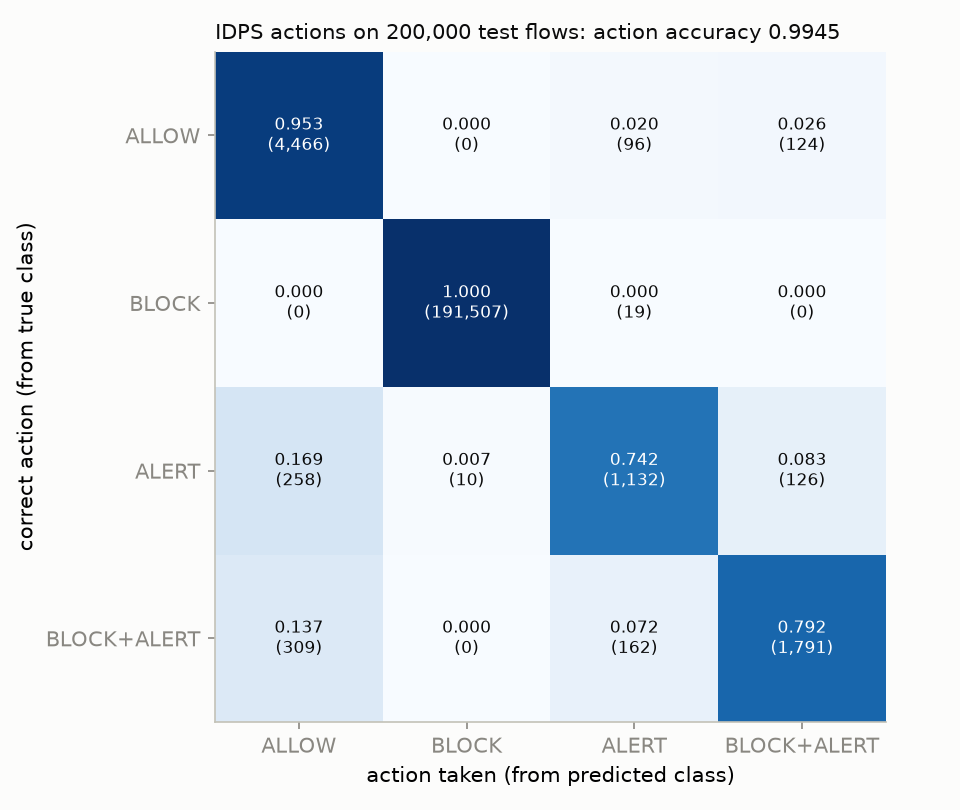
\includegraphics[width=0.9\columnwidth]{fig_idps_actions.png}
\caption{IDPS: correct action vs action taken on \idsRows{} test flows. Source: \texttt{results/prevention/summary.json}.}
\label{fig:idps}
\end{figure}

%=====================================================================
\section{Discussion}
A model that beats the benchmark by reading IAT is reading \emph{when} a capture was recorded. In a real
network, attacks are not scheduled into separate capture sessions, so this signal would not exist and the
learned rule would not transfer. The same reasoning applies to twins (N1) and file-level artifacts (N2, N5):
they reward memorising a capture rather than recognising an attack. For deployment we therefore use the
no-IAT model. Its 8-class macro-F1 (\vfDMfEight{}) is lower than the headline numbers, but it does not depend on
capture timing, and at the action level (where DoS and DDoS need the same response) it is accurate
(\idsActAcc{}). We recommend that results on CICIoT2023 report a file-grouped split and an IAT ablation next to
the shuffled-split numbers.

%=====================================================================
\section{Limitations and Future Work}
\textbf{Limitations.} (i) The 46-feature experiments use a public Kaggle subset of \vfRows{} rows, not the full
release, and we could not verify how it was sampled. (ii) CICIoT2023 has no IP addresses, so blocking is
simulated with placeholder IPs and generated rules. (iii) All results come from one dataset and one testbed.
(iv) Some early runs did not record validation metrics (marked [MISSING] in the appendix). (v) Our claim about
the paper's use of IAT is inferred from its stated pipeline (N7), not from re-running its code.

\textbf{Future work.} Re-extract features from the original pcaps with a corrected IAT; evaluate under
file-grouped and cross-dataset splits; add aggregate (multi-flow) features to separate DoS from DDoS; test the
IDPS on live traffic with real addresses.

%=====================================================================
\section{Conclusion}
On CICIoT2023, the gap between ``beats the benchmark'' and ``detects attacks'' comes from the evaluation, not
the model. With validation-only selection we beat the published 8-class macro-F1 on the full release and all
targets on a 46-feature subset, but the subset results rest largely on IAT, which behaves like a capture
timestamp, and shuffled splits contain heavy duplication. A no-IAT model ties or beats the paper only on the
multi-class macro-F1 targets, and wrapped in a prevention layer it chooses the right action for \idsActAcc{}
of unseen flows at about \idsLatSingle{}\,ms per flow.

\bibliographystyle{IEEEtran}
\bibliography{refs}

%=====================================================================
\onecolumn
\appendix
\section*{Appendix: every trained model}
All rows are generated by \texttt{paper/tools/build\_facts.py} from the JSON file listed in
\texttt{paper/data/all\_models.json}. Numbers not recorded in the JSONs are marked [MISSING]; the full list is
in \texttt{paper/data/missing.json}.
{\tiny
\begin{longtable}{llrp{3.2cm}p{4.4cm}rrrrr}
\caption{Every model trained in this project (v1-v4). Val = validation split, mF1 = macro-F1. n/a: no separate validation (train+val run, or test-only push run). n/r = not recorded during the original run.}\label{tab:allmodels}\\
\toprule
\textbf{Ver} & \textbf{Data} & \textbf{Task} & \textbf{Model} & \textbf{Config} & \textbf{Val acc} & \textbf{Val mF1} & \textbf{Test acc} & \textbf{Test mF1} & \textbf{Train s} \\
\midrule
\endfirsthead
\toprule
\textbf{Ver} & \textbf{Data} & \textbf{Task} & \textbf{Model} & \textbf{Config} & \textbf{Val acc} & \textbf{Val mF1} & \textbf{Test acc} & \textbf{Test mF1} & \textbf{Train s} \\
\midrule
\endhead
v1 & full 39f & 2 & catboost\_balanced & depth=10, lr=0.1, iters=3000, w=Balanced & 0.9863 & 0.8834 & 0.9864 & 0.8840 & 111 \\
v1 & full 39f & 2 & lightgbm\_cfg1 & leaves=255, lr=0.1 & 0.9937 & 0.9314 & 0.9937 & 0.9319 & 1,810 \\
v1 & full 39f & 2 & lightgbm\_cfg2 & leaves=512, lr=0.05 & 0.9937 & 0.9323 & 0.9938 & 0.9328 & 3,465 \\
v1 & full 39f & 2 & lightgbm\_cfg3\_weighted & leaves=512, lr=0.05, sqrt class weights & 0.9921 & 0.9229 & 0.9921 & 0.9236 & 7,975 \\
v1 & full 39f & 2 & mlp\_v1 & layers=1024-512-256 & 0.9883 & 0.8962 & 0.9884 & 0.8967 & 2,008 \\
v1 & full 39f & 2 & xgboost\_cfg1 & depth=12, lr=0.1 & 0.9934 & 0.9286 & 0.9934 & 0.9295 & 37 \\
v1 & full 39f & 2 & xgboost\_cfg2 & leaves=1024, lr=0.05 & 0.9935 & 0.9303 & 0.9936 & 0.9313 & 115 \\
v1 & full 39f & 2 & xgboost\_cfg3\_weighted & leaves=1024, lr=0.05, sqrt class weights & 0.9903 & 0.9102 & 0.9903 & 0.9106 & 499 \\
v1 & full 39f & 8 & catboost\_balanced & depth=10, lr=0.1, iters=3000, w=Balanced & 0.7454 & 0.6324 & 0.7451 & 0.6333 & 167 \\
v1 & full 39f & 8 & lightgbm\_cfg1 & leaves=255, lr=0.1 & 0.8613 & 0.6629 & 0.8610 & 0.6672 & 818 \\
v1 & full 39f & 8 & lightgbm\_cfg2 & leaves=512, lr=0.05 & 0.8634 & 0.6899 & 0.8633 & 0.6923 & 2,921 \\
v1 & full 39f & 8 & lightgbm\_cfg3\_weighted & leaves=512, lr=0.05, sqrt class weights & 0.8407 & 0.7283 & 0.8403 & 0.7305 & 22,199 \\
v1 & full 39f & 8 & mlp\_v1 & layers=1024-512-256 & 0.8334 & 0.6940 & 0.8330 & 0.6976 & 1,807 \\
v1 & full 39f & 8 & xgboost\_cfg1 & depth=12, lr=0.1 & 0.8645 & 0.7123 & 0.8642 & 0.7129 & 750 \\
v1 & full 39f & 8 & xgboost\_cfg2 & leaves=1024, lr=0.05 & 0.8652 & 0.7166 & 0.8650 & 0.7168 & 9,577 \\
v1 & full 39f & 8 & xgboost\_cfg3\_weighted & leaves=1024, lr=0.05, sqrt class weights & 0.8415 & 0.7282 & 0.8410 & 0.7324 & 10,626 \\
v1 & full 39f & 34 & catboost\_balanced & depth=10, lr=0.1, iters=3000, w=Balanced & 0.7425 & 0.5125 & 0.7423 & 0.5130 & 101 \\
v1 & full 39f & 34 & lightgbm\_cfg1 & leaves=255, lr=0.1 & 0.7847 & 0.5458 & 0.7845 & 0.5460 & 2,362 \\
v1 & full 39f & 34 & lightgbm\_cfg2 & leaves=512, lr=0.05 & 0.7886 & 0.5698 & 0.7886 & 0.5703 & 5,205 \\
v1 & full 39f & 34 & lightgbm\_cfg3\_weighted & leaves=512, lr=0.05, sqrt class weights & 0.7893 & 0.6137 & 0.7891 & 0.6158 & 7,866 \\
v1 & full 39f & 34 & mlp\_v1 & layers=1024-512-256 & 0.7827 & 0.6111 & 0.7827 & 0.6140 & 1,886 \\
v1 & full 39f & 34 & xgboost\_cfg1 & depth=12, lr=0.1 & 0.7959 & 0.6323 & 0.7958 & 0.6352 & 944 \\
v1 & full 39f & 34 & xgboost\_cfg2 & leaves=1024, lr=0.05 & 0.7977 & 0.6349 & 0.7975 & 0.6369 & 2,158 \\
v1 & full 39f & 34 & xgboost\_cfg3\_weighted & leaves=1024, lr=0.05, sqrt class weights & 0.7939 & 0.6398 & 0.7939 & 0.6423 & 13,137 \\
v2 & full 39f & 2 & accpush\_xgb\_ensemble\_threshold & - & n/a & n/a & 0.9934 & 0.9318 & n/r \\
v2 & full 39f & 2 & accpush\_xgboost\_deep\_low\_lr & depth=16, lr=0.02 & n/a & n/a & 0.9936 & 0.9314 & 126 \\
v2 & full 39f & 2 & accpush\_xgboost\_lossguide\_wide & leaves=2048, lr=0.02 & n/a & n/a & 0.9936 & 0.9314 & 467 \\
v2 & full 39f & 2 & random\_forest & trees=200 & n/r & n/r & 0.9933 & 0.9271 & 320 \\
v2 & full 39f & 2 & rf\_balanced & trees=100, w=balanced\_subsample & n/r & n/r & 0.9928 & 0.9219 & 284 \\
v2 & full 39f & 2 & xgboost\_balanced\_deep & depth=14, lr=0.05, sqrt class weights & 0.9927 & 0.9268 & 0.9927 & 0.9272 & 535 \\
v2 & full 39f & 2 & xgboost\_deep & depth=16, lr=0.03 & 0.9935 & 0.9302 & 0.9936 & 0.9313 & 246 \\
v2 & full 39f & 2 & xgboost\_trainval & leaves=1024, lr=0.05 & n/a & n/a & 0.9936 & 0.9314 & 1,901 \\
v2 & full 39f & 8 & random\_forest & trees=200 & n/r & n/r & 0.8587 & 0.6978 & 768 \\
v2 & full 39f & 8 & rf\_balanced & trees=100, w=balanced\_subsample & n/r & n/r & 0.7759 & 0.6998 & 664 \\
v2 & full 39f & 8 & xgboost\_balanced\_deep & depth=14, lr=0.05, sqrt class weights & 0.8419 & 0.7295 & 0.8415 & 0.7308 & 1,414 \\
v2 & full 39f & 8 & xgboost\_deep & depth=16, lr=0.03 & 0.8653 & 0.7156 & 0.8650 & 0.7159 & 2,054 \\
v2 & full 39f & 8 & xgboost\_trainval & leaves=1024, lr=0.05 & n/a & n/a & 0.8649 & 0.7172 & 6,675 \\
v2 & full 39f & 34 & random\_forest & trees=200 & n/r & n/r & 0.7891 & 0.6233 & 736 \\
v2 & full 39f & 34 & rf\_balanced & trees=100, w=balanced\_subsample & n/r & n/r & 0.7737 & 0.6244 & 661 \\
v2 & full 39f & 34 & xgboost\_balanced\_deep & depth=14, lr=0.05, sqrt class weights & 0.7945 & 0.6401 & 0.7944 & 0.6420 & 4,137 \\
v2 & full 39f & 34 & xgboost\_balanced\_p025 & depth=12, lr=0.05, w-power=0.25 & n/r & n/r & 0.7974 & 0.6412 & 7,419 \\
v2 & full 39f & 34 & xgboost\_balanced\_p050 & depth=12, lr=0.05, w-power=0.5 & n/r & 0.6412 & 0.7946 & 0.6429 & 4,440 \\
v2 & full 39f & 34 & xgboost\_deep & depth=16, lr=0.03 & 0.7977 & 0.6345 & 0.7977 & 0.6379 & 5,643 \\
v2 & full 39f & 34 & xgboost\_deep\_balanced & depth=16, lr=0.03, w-power=0.5 & n/r & n/r & 0.7941 & 0.6416 & 4,589 \\
v2 & full 39f & 34 & xgboost\_trainval & leaves=1024, lr=0.05 & n/a & n/a & 0.7980 & 0.6377 & 12,618 \\
v3 & full 39f & 2 & catboost\_c1\_bal\_s42 & depth=10, lr=0.08, iters=1500, w=bal & 0.9926 & 0.9207 & 0.9926 & 0.9213 & 14 \\
v3 & full 39f & 2 & catboost\_c1\_none\_s1 & depth=10, lr=0.08, iters=1500, w=none & 0.9928 & 0.9230 & 0.9928 & 0.9232 & 22 \\
v3 & full 39f & 2 & catboost\_c1\_none\_s2 & depth=10, lr=0.08, iters=1500, w=none & 0.9927 & 0.9213 & 0.9927 & 0.9219 & 13 \\
v3 & full 39f & 2 & catboost\_c1\_none\_s42 & depth=10, lr=0.08, iters=1500, w=none & 0.9927 & 0.9212 & 0.9927 & 0.9217 & 14 \\
v3 & full 39f & 2 & catboost\_c2\_bal\_s42 & depth=8, lr=0.05, iters=2000, w=bal & 0.9924 & 0.9185 & 0.9925 & 0.9192 & 11 \\
v3 & full 39f & 2 & catboost\_c2\_none\_s42 & depth=8, lr=0.05, iters=2000, w=none & 0.9926 & 0.9201 & 0.9926 & 0.9207 & 14 \\
v3 & full 39f & 34 & catboost\_c1\_bal\_s42 & depth=10, lr=0.08, iters=1500, w=bal & 0.7687 & 0.5010 & 0.7688 & 0.5006 & 42 \\
v3 & full 39f & 34 & catboost\_c1\_none\_s1 & depth=10, lr=0.08, iters=1500, w=none & 0.7746 & 0.5411 & 0.7749 & 0.5415 & 41 \\
v3 & full 39f & 34 & catboost\_c1\_none\_s2 & depth=10, lr=0.08, iters=1500, w=none & 0.7746 & 0.5415 & 0.7749 & 0.5417 & 39 \\
v3 & full 39f & 34 & catboost\_c1\_none\_s42 & depth=10, lr=0.08, iters=1500, w=none & 0.7747 & 0.5395 & 0.7750 & 0.5393 & 41 \\
v3 & full 39f & 34 & catboost\_c2\_bal\_s42 & depth=8, lr=0.05, iters=2000, w=bal & 0.7637 & 0.4845 & 0.7638 & 0.4840 & 51 \\
v3 & full 39f & 34 & catboost\_c2\_none\_s42 & depth=8, lr=0.05, iters=2000, w=none & 0.7727 & 0.5256 & 0.7730 & 0.5261 & 37 \\
v3 & full 39f & 34 & catboost\_c2\_none\_s42\_b1024 & depth=8, lr=0.05, iters=2000, w=none & 0.7715 & 0.5199 & 0.7717 & 0.5202 & 48 \\
v3 & full 39f & 34 & hierarchical\_8to34\_hard\_s1 & stage1 xgb cfg3\_weighted + 6 family experts & 0.7717 & 0.6304 & 0.7714 & 0.6352 & 38 \\
v3 & full 39f & 34 & hierarchical\_8to34\_hard\_s2 & stage1 xgb cfg3\_weighted + 6 family experts & 0.7718 & 0.6296 & 0.7715 & 0.6351 & 37 \\
v3 & full 39f & 34 & hierarchical\_8to34\_hard\_s42 & stage1 xgb cfg3\_weighted + 6 family experts & 0.7717 & 0.6317 & 0.7714 & 0.6354 & 36 \\
v3 & full 39f & 34 & xgboost\_focal\_s42 & depth=12, lr=0.05, focal-gamma=2.0, w=sqrt-bal & 0.6595 & 0.5160 & 0.6597 & 0.5152 & 2,947 \\
v4 & Kaggle & 2 & rf [38f-noIAT] & trees=200 & 0.9944 & 0.9404 & 0.9945 & 0.9417 & 181 \\
v4 & Kaggle & 2 & rf [38f] & trees=200 & 0.9971 & 0.9685 & 0.9972 & 0.9696 & 154 \\
v4 & Kaggle & 2 & rf [46f-noIAT] & trees=200 & 0.9954 & 0.9513 & 0.9955 & 0.9523 & 186 \\
v4 & Kaggle & 2 & rf [46f] & trees=200 & 0.9976 & 0.9744 & 0.9977 & 0.9754 & 177 \\
v4 & Kaggle & 2 & xgb\_best [38f-noIAT] & leaves=1024, lr=0.05 & 0.9946 & 0.9429 & 0.9947 & 0.9436 & 251 \\
v4 & Kaggle & 2 & xgb\_best [38f] & leaves=1024, lr=0.05 & 0.9965 & 0.9632 & 0.9967 & 0.9652 & 44 \\
v4 & Kaggle & 2 & xgb\_best [46f-noIAT] & leaves=1024, lr=0.05 & 0.9959 & 0.9566 & 0.9959 & 0.9562 & 284 \\
v4 & Kaggle & 2 & xgb\_best [46f] & leaves=1024, lr=0.05 & 0.9974 & 0.9720 & 0.9974 & 0.9723 & 44 \\
v4 & Kaggle & 2 & xgb\_unw [38f] & depth=12, lr=0.1 & 0.9963 & 0.9602 & 0.9964 & 0.9618 & 9 \\
v4 & Kaggle & 2 & xgb\_unw [46f] & depth=12, lr=0.1 & 0.9972 & 0.9696 & 0.9972 & 0.9696 & 12 \\
v4 & Kaggle & 8 & rf [38f-noIAT] & trees=200 & 0.9064 & 0.7206 & 0.9061 & 0.7074 & 339 \\
v4 & Kaggle & 8 & rf [38f] & trees=200 & 0.9959 & 0.8806 & 0.9960 & 0.8758 & 228 \\
v4 & Kaggle & 8 & rf [46f-noIAT] & trees=200 & 0.9170 & 0.7306 & 0.9168 & 0.7193 & 389 \\
v4 & Kaggle & 8 & rf [46f] & trees=200 & 0.9962 & 0.8639 & 0.9963 & 0.8681 & 248 \\
v4 & Kaggle & 8 & xgb\_best [38f-noIAT] & leaves=1024, lr=0.05, w-power=0.5 & 0.9075 & 0.7419 & 0.9076 & 0.7346 & 934 \\
v4 & Kaggle & 8 & xgb\_best [38f] & leaves=1024, lr=0.05, w-power=0.5 & 0.9962 & 0.8823 & 0.9961 & 0.8799 & 207 \\
v4 & Kaggle & 8 & xgb\_best [46f-noIAT] & leaves=1024, lr=0.05, w-power=0.5 & 0.9156 & 0.7603 & 0.9154 & 0.7547 & 926 \\
v4 & Kaggle & 8 & xgb\_best [46f] & leaves=1024, lr=0.05, w-power=0.5 & 0.9968 & 0.8967 & 0.9967 & 0.8925 & 210 \\
v4 & Kaggle & 8 & xgb\_unw [38f] & leaves=1024, lr=0.05 & 0.9953 & 0.8219 & 0.9954 & 0.8138 & 232 \\
v4 & Kaggle & 8 & xgb\_unw [46f] & leaves=1024, lr=0.05 & 0.9960 & 0.8381 & 0.9960 & 0.8254 & 235 \\
v4 & Kaggle & 34 & rf [38f-noIAT] & trees=200 & 0.8844 & 0.6795 & 0.8842 & 0.6830 & 359 \\
v4 & Kaggle & 34 & rf [38f] & trees=200 & 0.9947 & 0.8082 & 0.9948 & 0.8011 & 249 \\
v4 & Kaggle & 34 & rf [46f-noIAT] & trees=200 & 0.8951 & 0.6951 & 0.8950 & 0.6959 & 380 \\
v4 & Kaggle & 34 & rf [46f] & trees=200 & 0.9949 & 0.7901 & 0.9950 & 0.7962 & 292 \\
v4 & Kaggle & 34 & xgb\_best [38f-noIAT] & depth=12, lr=0.05, w-power=0.5 & 0.8900 & 0.6969 & 0.8900 & 0.6979 & 358 \\
v4 & Kaggle & 34 & xgb\_best [38f] & depth=12, lr=0.05, w-power=0.5 & 0.9951 & 0.8291 & 0.9951 & 0.8361 & 293 \\
v4 & Kaggle & 34 & xgb\_best [46f-noIAT] & depth=12, lr=0.05, w-power=0.5 & 0.8973 & 0.7153 & 0.8976 & 0.7143 & 409 \\
v4 & Kaggle & 34 & xgb\_best [46f] & depth=12, lr=0.05, w-power=0.5 & 0.9957 & 0.8406 & 0.9957 & 0.8484 & 332 \\
v4 & Kaggle & 34 & xgb\_unw [38f] & depth=12, lr=0.05 & 0.9940 & 0.7780 & 0.9941 & 0.7819 & 349 \\
v4 & Kaggle & 34 & xgb\_unw [46f] & depth=12, lr=0.05 & 0.9946 & 0.7926 & 0.9947 & 0.7907 & 363 \\
\bottomrule
\end{longtable}
}


\section*{Numbers marked [MISSING]}
These values were looked for and not found in any result JSON:
\begin{itemize}\footnotesize
\item val metrics random\_forest (2-class) (\texttt{results/2\_class/random\_forest/results.json})
\item val metrics rf\_balanced (2-class) (\texttt{results/2\_class/rf\_balanced/results.json})
\item val metrics random\_forest (8-class) (\texttt{results/8\_class/random\_forest/results.json})
\item val metrics rf\_balanced (8-class) (\texttt{results/8\_class/rf\_balanced/results.json})
\item val metrics random\_forest (34-class) (\texttt{results/34\_class/random\_forest/results.json})
\item val metrics rf\_balanced (34-class) (\texttt{results/34\_class/rf\_balanced/results.json})
\item val metrics xgboost\_balanced\_p025 (34-class) (\texttt{results/34\_class/xgboost\_balanced\_p025/results.json})
\item val metrics xgboost\_balanced\_p050 (34-class) (\texttt{results/34\_class/xgboost\_balanced\_p050/results.json})
\item val metrics xgboost\_deep\_balanced (34-class) (\texttt{results/34\_class/xgboost\_deep\_balanced/results.json})
\item training time accpush\_xgb\_ensemble\_threshold (2-class) (\texttt{results/2\_class/accuracy\_push/results.json})
\end{itemize}


\end{document}
